\pdfobjcompresslevel=0
\pdfminorversion=9
\documentclass[aspectratio=169]{beamer}

\usepackage[utf8]{inputenc}

\setbeamersize{text margin left=3mm,text margin right=3mm} 

\usepackage{tabularray}
\usetheme{Oxygen}
\usepackage{graphicx}
\usepackage{hyperref}
%\usepackage{movie15}
\usepackage{textpos}
\usepackage{fancybox}
\usepackage{colortbl}
\usepackage{rotating}
\usepackage{subfigure}
%\usepackage{subcaption}
\usepackage{multicol}
\usepackage{multirow}
\usepackage{amsmath,amssymb,amsfonts,amsbsy,dsfont}
\usepackage{mathrsfs}
\usepackage{amsthm}
\usepackage{bm}
\usepackage{array}
%\usepackage[caption=false]{subfig}
\usepackage{arydshln}
\usepackage{breakcites}
\usepackage{booktabs}
\usepackage{amsmath, amssymb}
\usepackage{tikz}
\usetikzlibrary{angles,quotes}
 \usetikzlibrary{angles,quotes}
\usetikzlibrary{decorations.pathreplacing}
\usepackage{ragged2e}
\usetikzlibrary{positioning,mindmap,arrows.meta,bending}
\usetikzlibrary{mindmap, backgrounds, calc}
\usepackage{xcolor}

\usepackage{tabularray}
\usepackage{tabularx}
% Mindmap drawing library 
\usetikzlibrary{positioning,shapes,shadows,arrows, shapes.geometric}
\usepackage{adjustbox}

\let\oldcite\cite % store the original \cite command
\renewcommand{\cite}[1]{{\tiny\oldcite{#1}}}

\usepackage{bm}
\providecommand{\mat}[1]{{\bm{#1}}} 
\providecommand{\ve}[1]{{\bm{#1}}} 


\newcommand{\x}{\negthinspace\times\negthinspace}
\usepackage{etoolbox}

\DeclareUnicodeCharacter{2212}{-}

\usepackage{graphicx,xifthen,xstring} % <— necesario

\newif\iffigdraft
% \figdrafttrue   % ← modo rápido (150 dpi)
\figdraftfalse    % ← modo final (300 dpi)
\usepackage{booktabs,tabularx,colortbl}
\usepackage{amssymb} % para \checkmark

% Colores de filas
\definecolor{completed}{RGB}{232,246,239} % verde muy claro
\definecolor{writing}{RGB}{255,237,213}   % naranja muy claro

% Marcas usadas en la leyenda / celdas
\newcommand{\cmark}{\checkmark}
\newcommand{\wmark}{\textbf{W}} % o cambia por lo que prefieras
\newcommand{\rasterpdffile}[3][]{%
  % Uso: \rasterpdffile[<dpi>]{ruta/figura.pdf}{<ancho>}
  \def\dpi{#1}%
  \ifthenelse{\isempty{#1}}{\iffigdraft\def\dpi{150}\else\def\dpi{300}\fi}{}%
  \StrBefore{#2}{.pdf}[\base]%
  \IfFileExists{\base.ras@\dpi.png}{}{%
    \immediate\write18{gs -q -dSAFER -dBATCH -dNOPAUSE -sDEVICE=pngalpha -r\dpi
      -dFirstPage=1 -dLastPage=1 -o "\base.ras@\dpi.png" "#2"}%
  }%
  \includegraphics[width=#3]{\base.ras@\dpi.png}%
}

\usepackage[nopar]{lipsum} 

\newif\ifcomment
\newcommand{\Com}{\par\footnotesize\itshape\commenttrue}

\newenvironment{Itemize}
 {%
  \edef\Itemizecurrent{\the\font}%
  \itemize
  \preto{\item}{\ifcomment\par\Itemizecurrent\fi}%
 }{%
  \enditemize
 }

\newcommand{\Real}{\mathbb{R}}
\newcommand{\N}{\mathbb{N}}
%\newcommand{\Z}{\mathbb{Z}}
\newcommand{\unos}{\ve{1}}
\providecommand{\kernel}[2]


\definecolor{mypink1}{rgb}{0.858, 0.188, 0.478}


%%%%%%%%%%%%%%%%%%%%%%%%%%%%%%%%%%%%%%%%%%%%%%%%%%%%%%
%%%%%%%


\title[An Explainable Deep Learning Framework for Conditional Domain Adaptation | D.A. Pérez Rosero] {An Explainable Deep Learning Framework \\
for Conditional Domain Adaptation }
% \title[RiceClimaRemote ]{An interpretable  deep learning-based framework to support the analysis  of rice irrigation practices}
%\vspace{-0.3cm}
\author[D.A. Pérez Rosero] {}
\institute{\small{Diego Armando Pérez Rosero}\\
{\small\textbf{ Advisor:} Prof. Andrés Marino Álvarez-Meza}\\
{\small \textbf{Co-Advisor:} Prof. César Germán Castellanos Domínguez\\ 
 }
 
 
 
\includegraphics[width=0.12\textwidth]{EscudoUN.png}\\
 
 \scriptsize{
Universidad Nacional de Colombia \\ Signal Processing and Recognition Group - SPRG \\ Manizales, Colombia 
%Advisor:\\
%Co-advisor: César Germán Castellanos Domíguez, Ph.D.\\
\vspace{-0.3cm}
}}
\date[]{\scriptsize{\today}}

\setbeamercovered{dynamic}
\setbeamertemplate{navigation symbols}{}



\begin{document}

{\setbeamertemplate{headline}{}
\setbeamertemplate{footline}{}
\begin{frame}{}
\vspace{-0.7cm}
    \titlepage 
\end{frame}
}


\frame
{ \frametitle{Outline}
{\small 
  \tableofcontents[]}
}

\AtBeginSection[]
{
  \begin{frame}
  \frametitle{Outline}
  \tableofcontents[currentsection]
  \end{frame}
}



%%%%%%%%%%%%%%%%%%%%%%%%%%%%%%%%%%%%%%%%%
\section[Motivation]{Motivation}

\begin{frame}
\frametitle{Learning Paradigms}

\begin{figure}[h!]
\centering

\begin{columns}[T]
    % ---------- (a) Supervised ----------
    \column{0.33\textwidth}
    \centering
    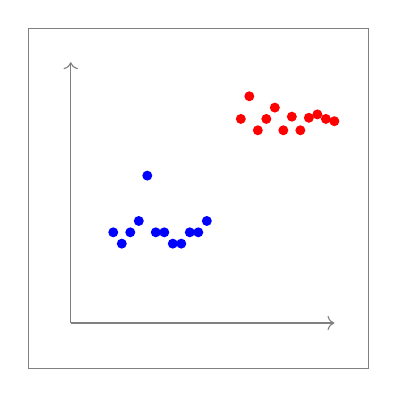
\begin{tikzpicture}[x=1.2cm,y=1.6cm, scale=0.9]
      % Marco y ejes
      \draw[gray] (0,0) rectangle (4,3);
      \draw[->,gray] (0.5,0.4) -- (0.5,2.7);
      \draw[->,gray] (0.5,0.4) -- (3.6,0.4);

      % --- Grupo 1 (Azul) ---
      \foreach \p in {
        (1.0,1.2), (1.1,1.1), (1.2,1.2), (1.3,1.3), (1.4,1.7),
        (1.5,1.2), (1.6,1.2), (1.7,1.1), (1.8,1.1), (1.9,1.2),
        (2.0,1.2), (2.1,1.3)
      }
        \fill[blue] \p circle (2pt);

      % --- Grupo 2 (Rojo) ---
      \foreach \p in {
        (2.5,2.2), (2.6,2.4), (2.7,2.1), (2.8,2.2), (2.9,2.3),
        (3.0,2.1), (3.1,2.22), (3.2,2.1), (3.3,2.21), (3.4,2.24),
        (3.5,2.20), (3.6,2.18)
      }
        \fill[red] \p circle (2pt);
    \end{tikzpicture}
    \textbf{\\ (a) Supervised}

    % ---------- (b) Semi-Supervised ----------
    \column{0.33\textwidth}
    \centering
    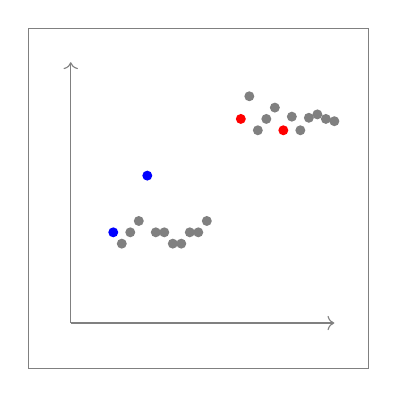
\begin{tikzpicture}[x=1.2cm,y=1.6cm, scale=0.9]
      % Marco y ejes
      \draw[gray] (0,0) rectangle (4,3);
      \draw[->,gray] (0.5,0.4) -- (0.5,2.7);
      \draw[->,gray] (0.5,0.4) -- (3.6,0.4);

      % --- Grupo 1 (Etiquetados - Azul) ---
      \fill[blue] (1.0,1.2) circle (2pt);
      \fill[blue] (1.4,1.7) circle (2pt);
      
      % --- Grupo 2 (Etiquetados - Rojo) ---
      \fill[red] (2.5,2.2) circle (2pt);
      \fill[red] (3.0,2.1) circle (2pt);

      % --- Datos no etiquetados (Gris) ---
      \foreach \p in {
        (1.1,1.1), (1.2,1.2), (1.3,1.3),
        (1.5,1.2), (1.6,1.2), (1.7,1.1), (1.8,1.1), (1.9,1.2),
        (2.0,1.2), (2.1,1.3), (2.6,2.4), (2.7,2.1), (2.8,2.2), (2.9,2.3),
        (3.1,2.22), (3.2,2.1), (3.3,2.21), (3.4,2.24),
        (3.5,2.20), (3.6,2.18)
      }
        \fill[gray] \p circle (2pt);
    \end{tikzpicture}
    \textbf{\\ (b) Semi-Supervised}

    % ---------- (c) Unsupervised ----------
    \column{0.33\textwidth}
    \centering
    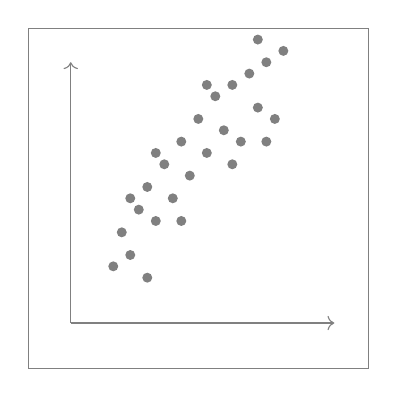
\begin{tikzpicture}[x=1.2cm,y=1.6cm, scale=0.9]
      % Marco y ejes
      \draw[gray] (0,0) rectangle (4,3);
      \draw[->,gray] (0.5,0.4) -- (0.5,2.7);
      \draw[->,gray] (0.5,0.4) -- (3.6,0.4);

      % --- Nube de puntos sin etiquetas ---
      \foreach \p in {
        (1.0,0.9), (1.1,1.2), (1.2,1.0), (1.3,1.4), (1.4,1.6),
        (1.5,1.3), (1.6,1.8), (1.7,1.5), (1.8,2.0), (1.9,1.7),
        (2.0,2.2), (2.1,1.9), (2.2,2.4), (2.3,2.1), (2.4,2.5),
        (2.5,2.0), (2.6,2.6), (2.7,2.3), (2.8,2.7), (2.9,2.2),
        (3.0,2.8), (1.2,1.5), (1.5,1.9), (1.8,1.3), (2.1,2.5),
        (2.4,1.8), (2.7,2.9), (1.4, 0.8), (2.8, 2.0)
      }
        \fill[gray] \p circle (2pt);
    \end{tikzpicture}
    \textbf{\\(c) Unsupervised}
\end{columns}

\end{figure}
\vfill
\centering
%Data patters  are extracted from fully labeled, partially labeled, or unlabeled data \cite{feng2023unsupervised}.
\textcolor{blue}{Data patterns can be extracted from fully and partially labeled or unlabeled data \cite{feng2023unsupervised}.}
\end{frame}





\begin{frame}{Training and Testing Distribution Shift}
\vspace{1cm}
\begin{figure}[H]
\centering
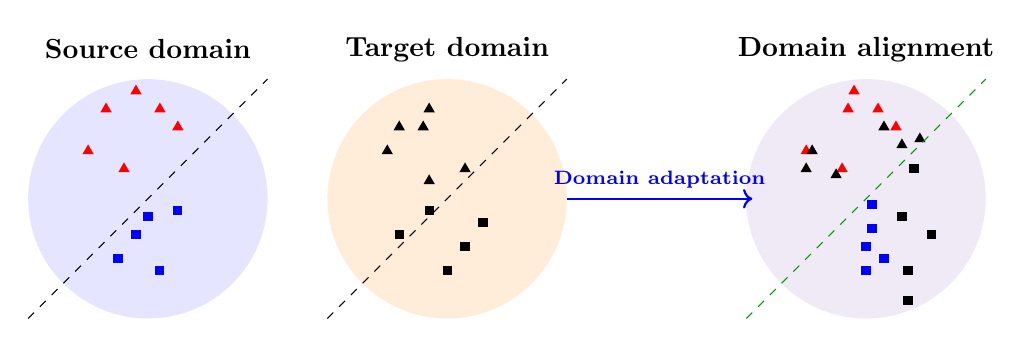
\begin{tikzpicture}[scale=0.76]

% Dominios desplazados -2 unidades
\fill[blue!10] (-8,0) circle (2cm); % Source
\fill[orange!15] (-3,0) circle (2cm); % Target
\fill[orange!15, opacity=0.6] (4,0) circle (2cm); % Target in alignment
\fill[blue!10, opacity=0.6] (4,0) circle (2cm); % Source in alignment

% Source Domain: Triángulos (rojos) y rectángulos (azules)
\foreach \x/\y in {-9/0.8, -8.7/1.5, -7.5/1.2, -8.2/1.8, -7.8/1.5, -8.4/0.5}
  \node[red!80!black, regular polygon, regular polygon sides=3, fill=red, scale=0.25] at (\x,\y) {};
\foreach \x/\y in {-7.5/-0.2, -8.2/-0.6, -8.5/-1.0, -8/-0.3, -7.8/-1.2}
  \node[blue!80!black, rectangle, fill=blue, scale=0.5] at (\x,\y) {};

% Target Domain: Triángulos y rectángulos (negros)
\foreach \x/\y in {-3.3/1.5, -3.4/1.2, -3.8/1.2, -4.0/0.8, -2.7/0.5, -3.3/0.3}
  \node[black, regular polygon, regular polygon sides=3, fill=black, scale=0.25] at (\x,\y) {};
\foreach \x/\y in {-2.4/-0.4, -3.8/-0.6, -3.0/-1.2, -2.7/-0.8, -3.3/-0.2}
  \node[black, rectangle, fill=black, scale=0.5] at (\x,\y) {};

% Alineación (mezcla de ambos dominios)
\foreach \x/\y in {3/0.8, 3.7/1.5, 4.5/1.2, 3.8/1.8, 4.2/1.5, 3.6/0.5}
  \node[red!80!black, regular polygon, regular polygon sides=3, fill=red, scale=0.25] at (\x,\y) {};
\foreach \x/\y in {4.0/-0.8, 4.3/-1.0, 4.0/-1.2, 4.1/-0.5,4.1/-0.1}
  \node[blue!80!black, rectangle, fill=blue, scale=0.5] at (\x,\y) {};
\foreach \x/\y in {3.1/0.8, 3.5/0.4, 3.0/0.5, 4.6/0.9, 4.3/1.2,4.9/1.0}
  \node[black, regular polygon, regular polygon sides=3, fill=black, scale=0.25] at (\x,\y) {};
\foreach \x/\y in {4.8/0.5, 4.6/-0.3, 4.7/-1.2,5.1/-0.6,4.7/-1.7 }
  \node[black, rectangle, fill=black, scale=0.5] at (\x,\y) {};

% Líneas divisorias corregidas
\draw[dashed] (-10,-2) -- (-6,2);
\draw[dashed] (-5,-2) -- (-1,2);
\draw[dashed, green!60!black] (2,-2) -- (6,2);

% Flecha de adaptación
\draw[->, thick, blue] (-1,0) -- (2.1,0)
  node[midway, above, text=blue, font=\bfseries\scriptsize] 
  {Domain adaptation};

% Títulos
\node at (-8,2.5) {\textbf{Source domain}};
\node at (-3,2.5) {\textbf{Target domain}};
\node at (4,2.5) {\textbf{Domain alignment}};

\end{tikzpicture}
\end{figure}
 

\vspace{0.7pt}

\centering
\color{blue}{
    Domain adaptation addresses performance degradation under distributional shift \cite{huang2023enhancing}.}


\end{frame}
%falta introducción
%falta GCPD 1 Slide
\begin{frame}{Model-Based Domain Alignment }
\begin{center}
\vspace{-0.65cm}
\begin{figure}[H]
\centering
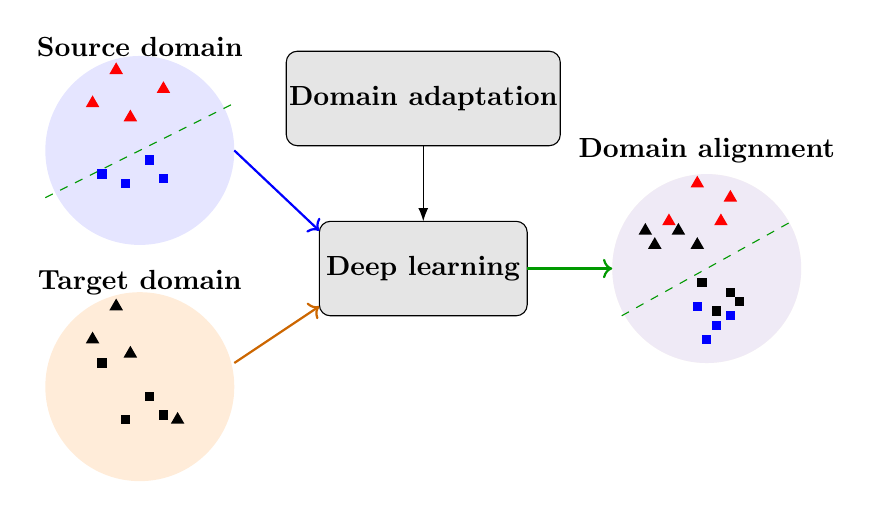
\begin{tikzpicture}[scale=0.6]

% Source domain (arriba)
\fill[blue!10] (-6,2.5) circle (2cm);
\node at (-6,4.7) {\textbf{Source domain}};
\foreach \x/\y in {-7/3.5, -5.5/3.8, -6.5/4.2, -6.2/3.2}
  \node[red!80!black, regular polygon, regular polygon sides=3, fill=red, scale=0.3] at (\x,\y) {};
\foreach \x/\y in {-6.8/2.0, -5.8/2.3, -6.3/1.8, -5.5/1.9}
  \node[blue!80!black, rectangle, fill=blue, scale=0.5] at (\x,\y) {};
% Línea divisoria en el Source domain
\draw[dashed,green!60!black] (-8,1.5) -- (-4,3.5);

% Target domain (abajo)
\fill[orange!15] (-6,-2.5) circle (2cm);
\node at (-6,-0.3) {\textbf{Target domain}};
\foreach \x/\y in {-7/-1.5, -5.2/-3.2, -6.5/-0.8, -6.2/-1.8}
  \node[black, regular polygon, regular polygon sides=3, fill=black, scale=0.3] at (\x,\y) {};
\foreach \x/\y in {-6.8/-2.0, -5.8/-2.7, -6.3/-3.2, -5.5/-3.1}
  \node[black, rectangle, fill=black, scale=0.5] at (\x,\y) {};

% Bloque Deep Learning
\draw[rounded corners, fill=gray!20, draw=black] (-2.2,-1) rectangle (2.2,1);
\node at (0,0) {\textbf{Deep learning}};

% --- Caja de Domain adaptation (encabezado) ---
\draw[rounded corners, fill=gray!20, draw=black] (-2.9,2.6) rectangle (2.9,4.6);
\node at (0,3.6) {\textbf{Domain adaptation}};
\draw[-Latex, thin] (0,2.6) -- (0,1); % flecha al bloque DL

% Domain Alignment (derecha)
\fill[orange!15, opacity=0.6] (6,0) circle (2cm);
\fill[blue!10,  opacity=0.6] (6,0) circle (2cm);
\node at (6,2.5) {\textbf{Domain alignment}};
\foreach \x/\y in {5.2/1.0, 6.5/1.5, 5.8/1.8, 6.3/1.0}
  \node[red!80!black, regular polygon, regular polygon sides=3, fill=red, scale=0.3] at (\x,\y) {};
\foreach \x/\y in {5.8/-0.8, 6.2/-1.2, 6.0/-1.5, 6.5/-1.0}
  \node[blue!80!black, rectangle, fill=blue, scale=0.5] at (\x,\y) {};
\foreach \x/\y in {4.9/0.5, 4.7/0.8, 5.4/0.8, 5.8/0.5}
  \node[black, regular polygon, regular polygon sides=3, fill=black, scale=0.3] at (\x,\y) {};
\foreach \x/\y in {5.9/-0.3, 6.5/-0.5, 6.2/-0.9, 6.7/-0.7}
  \node[black, rectangle, fill=black, scale=0.5] at (\x,\y) {};
% Línea divisoria en Domain alignment
\draw[dashed, green!60!black] (4.2,-1) -- (7.8,1);

% Flechas de conexión
\draw[->, thick, blue] (-4,2.5) -- (-2.2,0.8);
\draw[->, thick, orange!80!black] (-4,-2) -- (-2.2,-0.8);
\draw[->, thick, green!60!black] (2.2,0) -- (4,0);

\end{tikzpicture}
\end{figure}
\end{center}
\centering
\color{blue}{Models align source–target domains via learned features and distribution matching \cite{zhang2025domain}. }
\end{frame}

\begin{frame}{Signal Processing and Recognition Group - SPRG}
  \begin{columns}[T,onlytextwidth]
    \begin{column}{0.5\textwidth}
      \centering
      
\includegraphics[width=\linewidth]{Figures/Images.png}
      \vspace{2mm}
      \textbf{(a)} Computer vision applications
    \end{column}
    \begin{column}{0.5\textwidth}
      \centering
      
\includegraphics[width=\linewidth]{Figures/TDAH.png}
      \vspace{2mm}
      \textbf{(b)} EEG applications
    \end{column}
  \end{columns}
  \centering
  \textcolor{blue}{SPRG advances robust DL methods for EEG analysis and vision-based tasks.}
\end{frame}

% ------------------------------------

\begin{frame}{ ACEMATE}
\begin{columns}[T,totalwidth=\textwidth]

% -------- Left column: main image --------
\begin{column}{0.5\textwidth}
  \centering
  
\includegraphics[width=0.6\linewidth]{Figures/main.png}

\end{column}

% -------- Right column: partner entities (exactly two rows) --------
\vspace{4}
\begin{column}{0.5\textwidth}
  \centering

  % ==== Row 1: three logos ====
  
\includegraphics[height=1.8cm]{Figures/EscudoU.jpg}

\includegraphics[height=1.8cm]{Figures/autonoma.png}\\
  
\includegraphics[height=1.8cm]{Figures/logo-bios.png}

\includegraphics[height=1.8cm]{Figures/utp.jpg}\\
  
\includegraphics[height=1.8cm]{Figures/cruz_roja.png}
  
\includegraphics[height=1.8cm]{Figures/logo-umanizales.png}

\end{column}

\end{columns}
\begin{center}
    \textcolor{blue}{ADHD  analysis with serious games, EEG-BCI, and multimodal machine learning.}
\end{center}
\end{frame}




% \begin{frame}{Intra-Class and Intra-Subject Variability }
% \begin{center}
% \vspace{0.1cm}
% \begin{figure}[h!]
% \centering
% \begin{minipage}[b]{0.48\linewidth}
%     \centering
%     \rasterpdffile[240]{Figures/IntraImages.pdf}{\linewidth}
%     \vspace{2mm}
%     \textbf{(a)} Intra-class Variability.
% \end{minipage}
% \hfill
% \begin{minipage}[b]{0.48\linewidth}
%     \centering
%     \rasterpdffile[240]{Figures/Intra.pdf}{\linewidth}
%     \vspace{2mm}
%     \textbf{(b)} Intra-subject Variability.
% \end{minipage}
% \end{figure}
% \end{center}
% \vspace{-0.2cm}

% \centering \color{blue}{Intra-class and intra-subject variability hinder robust Domain Adaptation (DA)~\cite{li2025inter}.}
% \end{frame}
 
% \begin{frame}
% \frametitle{Inter-Class and Inter-Subject Variability}
% \begin{center}
% \vspace{-0.05 cm}
% \begin{figure}[h!]
% \centering
% \begin{minipage}[b]{0.48\linewidth}
%     \centering
%     \rasterpdffile[240]{Figures/InterImages.pdf}{\linewidth}
%     \vspace{2mm}
%     \textbf{(a)} Inter-class variability
% \end{minipage}
% \hfill
% \begin{minipage}[b]{0.48\linewidth}
%     \centering
%     \rasterpdffile[240]{Figures/Inter.pdf}{\linewidth}
%     \vspace{2mm}
%     \textbf{(b)} Inter-subject variability
% \end{minipage}
% \end{figure}
		
% 		\end{center}
% 		\centering \color{blue}{Inter-class$/$subject variability challenge model generalization in DA~\cite{wang2025bsan}.}
% \end{frame}

% \begin{frame}
% \frametitle{Cross-Datasets Variability}
  
%  \begin{center}
% \vspace{-0.05 cm}
% \begin{figure}[h!]
% \centering
% \begin{minipage}[b]{0.48\linewidth}
%     \centering
%     \rasterpdffile[240]{Figures/CrossImages.pdf}{\linewidth}
%     \vspace{2mm}
%     \textbf{(a)} Image datasets
% \end{minipage}
% \hfill
% \begin{minipage}[b]{0.48\linewidth}
%     \centering
%     \rasterpdffile[240]{Figures/Crossdata.pdf}{\linewidth}
%     \vspace{2mm}
%     \textbf{(b)} EEG datasets
% \end{minipage}
% \end{figure}
		
% 		\end{center}
% 	\centering\color{blue}{Cross-dataset heterogeneity hinders out-of-domain generalization  \cite{imtiaz2025towards}.}
  
% \end{frame}

\section{Problem Statement}

% \begin{frame}{Challenges in DA}

% \begin{figure}[H]
% \centering
% \begin{tikzpicture}[x=1cm,y=1cm,font=\footnotesize,line width=0.8pt]

% % --- parámetros base ---
% \def\Y{1.8}      % semialtura para mayor separación vertical
% \def\xLB{9.5}    % x de la llave izquierda (apunta hacia el centro)
% \def\xRB{0.5}    % x de la llave derecha (apunta hacia el centro)
% \def\xTxt{1.5}   % x de los textos intermedios

% % Llave izquierda (apunta hacia el centro)
% \draw[decorate,decoration={brace,raise=0pt,amplitude=4pt}]
%   (\xLB,\Y+1) -- (\xLB,-\Y-1);

% % Etiqueta izquierda con la cita más reciente
% \node[anchor=east,align=left] at (\xRB-0.2,0) {Domain\\Adaptation};

% % Textos intermedios (información de la imagen)
% \node[anchor=west,align=left] at (\xTxt,\Y)   {\textbf{Domain-Invariant Features} \\ Identifying and preserving features \\ that remain consistent across \\ different domains~\cite{ruan2021optimal}.};
% \node[anchor=west,align=left] at (\xTxt,0)    {\textbf{Discriminative Features} \\ Maintaining features that effectively \\ distinguish between different classes~\cite{kumar2025unified}.};
% \node[anchor=west,align=left] at (\xTxt,-\Y)  {\textbf{Model Interpretability} \\ Ensuring models are understandable \\ and transparent in their \\ decision-making~\cite{van2025model}.};

% % Llave derecha (apunta hacia el centro)
% \draw[decorate,decoration={brace,raise=0pt,amplitude=4pt}]
%   (\xRB,-\Y-1) -- (\xRB,\Y+1);

% % Salida en tres líneas
% \node[anchor=west,align=left] at (\xLB+0.2,0)
%   {Generalization to\\unseen domains};

% \end{tikzpicture}
% \end{figure}
% \begin{center}
%     \textcolor{blue}{Generalization to unseen domains constrains reliable deployment in practice \cite{vuong2025domain}.}

% \end{center}
% \end{frame}


\begin{frame}{Issue \#1: Preservation of Domain-Invariant Features}

\begin{figure}[H]
\centering
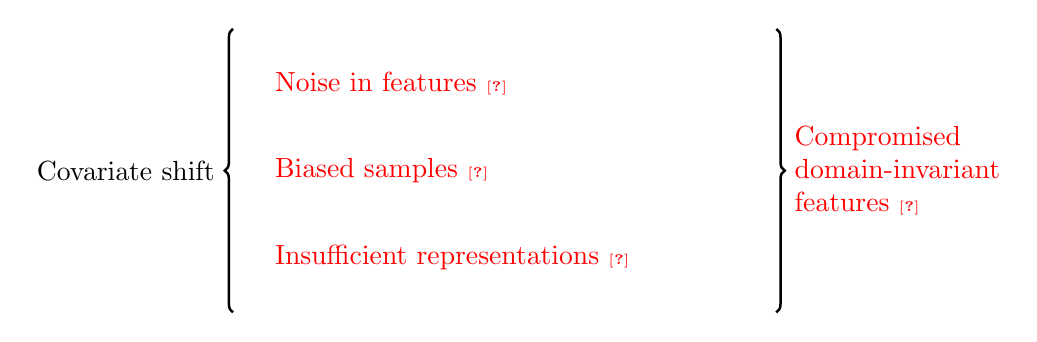
\begin{tikzpicture}[x=1cm,y=1cm,font=\normalsize,line width=0.9pt]

% --- parámetros ---
\def\Y{1.1}      % semialtura
\def\xLB{8.5}    % x llave derecha
\def\xRB{1.6}    % x llave izquierda
\def\xTxt{2.0}   % x de los textos (centrados entre llaves)

% Llave izquierda (apunta hacia el centro)
\draw[decorate,decoration={brace,raise=0pt,amplitude=3pt}]
  (\xLB,\Y+0.7) -- (\xLB,-\Y-0.7);

% Etiqueta izquierda (sin cita)
\node[anchor=east] at (1.5,0) {Covariate shift};

% Textos intermedios (sin líneas) — citas no repetidas y recientes de tu texto
\node[anchor=west] at (\xTxt,\Y)   {\textcolor{red}{Noise in features \cite{zhu2025fedweight}}};
\node[anchor=west] at (\xTxt,0)    {\textcolor{red}{Biased samples \cite{han2020towards}}};
\node[anchor=west] at (\xTxt,-\Y)  {\textcolor{red}{Insufficient representations \cite{zhao2019learning}}};

% Llave derecha (apunta hacia el centro)
\draw[decorate,decoration={brace,raise=0pt,amplitude=3pt}]
  (\xRB,-\Y-0.7) -- (\xRB,\Y+0.7);

% Salida en tres líneas (cita distinta a las anteriores)
\node[anchor=west,align=left] at (\xLB+0.1,0)
  { \textcolor{red}{Compromised}\\\textcolor{red}{domain-invariant}\\\textcolor{red}{features \cite{ruan2021optimal}}};

\end{tikzpicture}
\end{figure}

\begin{center}
\textcolor{blue}{Covariate shift increases overfitting and destabilizes deployment performance \cite{guo2022evaluation}.}
\end{center}

\end{frame}




\begin{frame}{Issue \#2: Maintenance of Discriminative Features}

\begin{figure}[H]
\centering
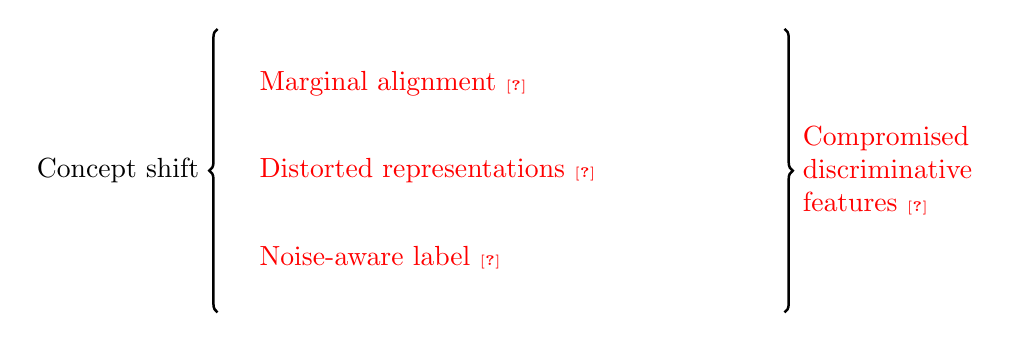
\begin{tikzpicture}[x=1cm,y=1cm,font=\normalsize,line width=0.9pt]

% --- parámetros base (consistentes con Issue #1) ---
\def\Y{1.1}      % semialtura
\def\xLB{8.8}    % x de la llave izquierda (apunta hacia el centro)
\def\xRB{1.6}    % x de la llave derecha (apunta hacia el centro)
\def\xTxt{2.0}   % x de los textos intermedios

% Llave izquierda (apunta hacia el centro)
\draw[decorate,decoration={brace,raise=0pt,amplitude=3pt}]
  (\xLB,\Y+0.7) -- (\xLB,-\Y-0.7);

% Etiqueta izquierda (sin cita)
\node[anchor=east] at (1.5,0) {Concept shift};

% Textos intermedios (sin líneas)
\node[anchor=west] at (\xTxt,\Y)   {\textcolor{red}{Marginal alignment \cite{tachet2020domain}}};
\node[anchor=west] at (\xTxt,0)    {\textcolor{red}{Distorted representations \cite{jiang2020implicit}}};
\node[anchor=west] at (\xTxt,-\Y)  {\textcolor{red}{Noise-aware label \cite{li2025addressing}}};

% Llave derecha (apunta hacia el centro)
\draw[decorate,decoration={brace,raise=0pt,amplitude=3pt}]
  (\xRB,-\Y-0.7) -- (\xRB,\Y+0.7);

% Salida en tres líneas
\node[anchor=west,align=left] at (\xLB+0.1,0)
  {\textcolor{red}{Compromised}\\\textcolor{red}{discriminative}\\\textcolor{red}{features \cite{kumar2025unified}}};
\end{tikzpicture}

\end{figure}

\begin{center}
\textcolor{blue}{Concept shift degrades class separability and increases misclassification risk \cite{kumar2025unified}.}
\end{center}
\end{frame}


\begin{frame}
\frametitle{EEG Variability Challenges}

\begin{figure}[h!]
\centering

\begin{columns}[T]
    % ---------- (a) Supervised ----------
    \column{0.33\textwidth}
    \centering
    \rasterpdffile[240]{Figures/Intra.pdf}{\linewidth}
    \textbf{\\ (a) Intra-subject variability}
    
    
    
    \column{0.33\textwidth}
    \centering
    \rasterpdffile[240]{Figures/Inter.pdf}{\linewidth}
    \textbf{\\ (b)Inter-subject variability}
    
    
    \column{0.33\textwidth}
    \centering
    \rasterpdffile[240]{Figures/Crossdata.pdf}{\linewidth}
    \textbf{\\(c) EEG datasets}
\end{columns}

\end{figure}
\vfill
\centering
%Data patters  are extracted from fully labeled, partially labeled, or unlabeled data \cite{feng2023unsupervised}.
\textcolor{blue}{EEG variability across subjects and datasets limits robust domain generalization~\cite{imtiaz2025towards}.}
\end{frame}

\begin{frame}{Issue \#3: Interpretability}

\begin{figure}[H]
\centering
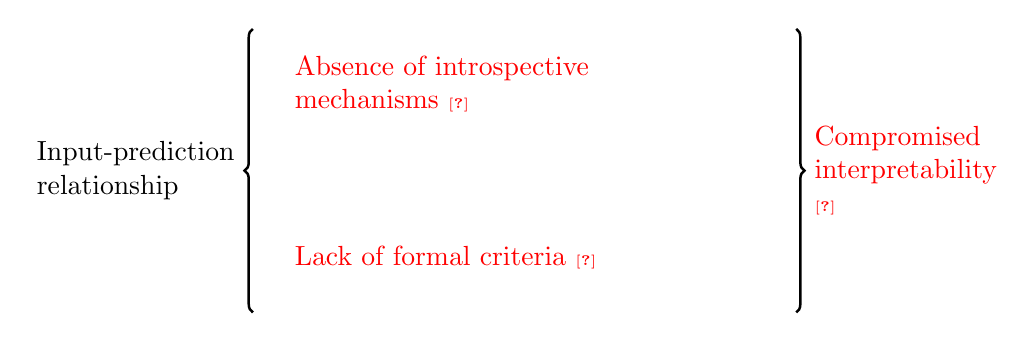
\begin{tikzpicture}[x=1cm,y=1cm,font=\normalsize,line width=0.9pt]

% --- parámetros base ---
\def\Y{1.1}
\def\xLB{8.5}
\def\xRB{1.6}
\def\xTxt{2.0}

% Llave izquierda (apunta hacia el centro)
\draw[decorate,decoration={brace,raise=0pt,amplitude=3pt}]
  (\xLB,\Y+0.7) -- (\xLB,-\Y-0.7);

% Etiqueta izquierda (sin cita)
\node[anchor=east,align=left] at (1.5,0) {Input-prediction\\relationship};

% Textos intermedios (sin líneas)
\node[anchor=west,align=left] at (\xTxt,\Y)
  {\textcolor{red}{Absence of introspective}\\ \textcolor{red}{mechanisms \cite{yuksel2025interpretability}}};
\node[anchor=west] at (\xTxt,-\Y)
  {\textcolor{red}{Lack of formal criteria \cite{xua2024interpretability}}};

% Llave derecha (apunta hacia el centro)
\draw[decorate,decoration={brace,raise=0pt,amplitude=3pt}]
  (\xRB,-\Y-0.7) -- (\xRB,\Y+0.7);

% Salida en dos líneas
\node[anchor=west,align=left] at (\xLB+0.1,0)
  {\textcolor{red}{Compromised}\\\textcolor{red}{interpretability}\\ \textcolor{red}{\cite{van2025model}}};

\end{tikzpicture}

\end{figure}
\begin{center}
\textcolor{blue}{ Insufficient interpretability conceals biases and undermines predictive reliability \cite{yuksel2025interpretability}.}
\end{center}

\end{frame}



\begin{frame}{Research Question}

\begin{itemize}
\justifying
    \item How to develop  a \textbf{class-conditional} \textbf{domain} \textbf{adaptation} framework, leveraging \textbf{noise-aware} labels, improve \textbf{generalization}, \textbf{discrimination}, and \textbf{interpretability} in \textbf{deep} \textbf{learning} under \textbf{covariate} \textbf{shift}?
\end{itemize}

\end{frame}

% \section{Background}
% % ===================== Slide 1: Geometría en espacios de Hilbert =====================
% \begin{frame}{Hilbert spaces}

% $\mathcal{H}$ Hilbert space over $\mathbb{K}\in\{\mathbb{R},\mathbb{C}\}$;
% $\langle \cdot,\cdot\rangle$ inner product; $\|\cdot\|:=\sqrt{\langle\cdot,\cdot\rangle}$ norm;
% $d(\mathbf{x},\mathbf{x}'):=\|\mathbf{x}-\mathbf{x}'\|$ metric;
% $\mathbf{x},\mathbf{x}',\mathbf{z}\in\mathcal{H}$; $a,b\in\mathbb{K}$.

% \medskip
% \textbf{Inner product axioms.}
% \[
% \langle a\mathbf{x}+b\mathbf{x}',\mathbf{z}\rangle
% = a\langle \mathbf{x},\mathbf{z}\rangle + b\langle \mathbf{x}',\mathbf{z}\rangle,\quad
% \langle \mathbf{x},\mathbf{x}'\rangle=\overline{\langle \mathbf{x}',\mathbf{x}\rangle},\quad
% \langle \mathbf{x},\mathbf{x}\rangle>0~(\mathbf{x}\neq \mathbf{0}).
% \]

% \medskip
% \textbf{Distance decomposition.}
% \[
% \|\mathbf{x}-\mathbf{x}'\|^{2}
% =\|\mathbf{x}\|^{2}-2\,\langle \mathbf{x},\mathbf{x}'\rangle+\|\mathbf{x}'\|^{2}.
% \]

% \medskip
% \textbf{Angle and orthogonality.}
% For nonzero vectors,
% \[
% \cos\bigl(\theta_{\mathbf{x}\mathbf{x}'}\bigr)
% =\frac{\langle \mathbf{x},\mathbf{x}'\rangle}{\|\mathbf{x}\|\,\|\mathbf{x}'\|},\qquad
% \langle \mathbf{x},\mathbf{x}'\rangle=0 \;\Longleftrightarrow\; \mathbf{x}\perp \mathbf{x}'.
% \]

% \medskip
% \footnotesize References: \cite{ryzhov2022modern}.
% % \end{frame}

% % ===================== Slide 2: Vista estocástica (L^2) =====================
% % ===================== Slide 2: L^2 — stochastic view =====================
% \begin{frame}{Stochastic Hilbert Spaces}

% From now on, we regard $(\chi,\mathcal{F},\mathbb{P})$ as the input space
% equipped with the push-forward measure $\mathbb{P}:=P_X$ induced by $X:\Omega\!\to\!\chi$. $L^{2}(\chi,\mathcal{F},\mathbb{P})=\{X:\mathbb{E}[X^{2}]<\infty\}$;
% random variables $X,Y:\chi\to\mathbb{R}$;
% inner product $\langle X,Y\rangle:=\mathbb{E}[XY]$; norm $\|X\|:=\sqrt{\mathbb{E}[X^{2}]}$.

% \medskip
% \textbf{Geometry of moments.}
% \[
% \mathbb{E}[X]=\langle X,1\rangle,\qquad
% \operatorname{Var}(X)=\|X-\mathbb{E}[X]\|^{2},
% \]
% \[
% \operatorname{Cov}(X,Y)=\langle X-\mathbb{E}[X],\,Y-\mathbb{E}[Y]\rangle,\qquad
% \rho(X,Y)=\frac{\operatorname{Cov}(X,Y)}{\sqrt{\operatorname{Var}(X)}\sqrt{\operatorname{Var}(Y)}}
% =\cos(\theta_{XY}).
% \]

% \medskip
% \textbf{Sample estimators (iid).}
% \[
% \widehat{\rho}(X,Y)
% =\frac{\tfrac{1}{M}\sum_{m=1}^{M}(x_m-\hat\mu_X)(y_m-\hat\mu_Y)}
% {\sqrt{\tfrac{1}{M}\sum_{m}(x_m-\hat\mu_X)^{2}}\,
%  \sqrt{\tfrac{1}{M}\sum_{m}(y_m-\hat\mu_Y)^{2}}}
% =\frac{\big\langle \mathbf{x}-\hat\mu_X\mathbf{1},\,\mathbf{y}-\hat\mu_Y\mathbf{1}\big\rangle_2}
% {\|\mathbf{x}-\hat\mu_X\mathbf{1}\|_2\,\|\mathbf{y}-\hat\mu_Y\mathbf{1}\|_2}.
% \]

% \medskip
% \footnotesize References: \cite{ash2000probability,wasserman2004all}.
% \end{frame}


% % ===================== Slide 3: RKHS — essentials =====================
% \begin{frame}{Reproducing Kernel Hilbert Space (RKHS)}

% On the same input/probability space $(\chi,\mathcal{F},\mathbb{P})$:
% kernel $\kappa:\chi\times\chi\to\mathbb{R}$ (symmetric, p.d.);
% RKHS $\mathcal{H}_{\kappa}$; feature map  with $\Phi:\chi\to\mathcal{H}_\kappa$.

% \medskip
% \textbf{Reproducing property.}
% For $f\in\mathcal{H}_{\kappa}$ and $\mathbf{x}\in\chi$:
% \[
% f(\mathbf{x})=\langle f,\kappa(\mathbf{x},\cdot)\rangle_{\mathcal{H}_{\kappa}}.
% \]

% \medskip
% \textbf{Kernel trick (geometry).}
% \[
% \kappa(\mathbf{x},\mathbf{x}')=\langle \Phi(\mathbf{x}),\Phi(\mathbf{x}')\rangle_{\mathcal{H}_{\kappa}}, 
% \quad \Phi(\mathbf{x}):=\kappa(\mathbf{x},\cdot), \quad
% \|\Phi(\mathbf{x})\|_{\mathcal{H}_{\kappa}}^{2}=\kappa(\mathbf{x},\mathbf{x}),
% \]
% \[
% \|\Phi(\mathbf{x})-\Phi(\mathbf{x}')\|_{\mathcal{H}_{\kappa}}^{2}
% =\kappa(\mathbf{x},\mathbf{x})-2\kappa(\mathbf{x},\mathbf{x}')+\kappa(\mathbf{x}',\mathbf{x}').
% \]

% \medskip
% \textbf{Angle and orthogonality (RKHS).}
% For nonzero feature vectors,
% \[
% \cos\!\bigl(\theta_{\Phi(\mathbf{x}),\Phi(\mathbf{x}')}\bigr)
% =\frac{\kappa(\mathbf{x},\mathbf{x}')}{\sqrt{\kappa(\mathbf{x},\mathbf{x})\,\kappa(\mathbf{x}',\mathbf{x')}}}\,,
% \qquad
% \kappa(\mathbf{x},\mathbf{x}')=0 \Longleftrightarrow \Phi(\mathbf{x})\perp \Phi(\mathbf{x}').
% \]

% \medskip
% \footnotesize References: \cite{scholkopf2018learning}.
% \end{frame}



% % ===================== Slide 4: $L^{2}(\Omega;\mathcal{H}_{\kappa})$ — stochastic RKHS view =====================
% \begin{frame}{Stochastic RKHS}

% Random variables $X,Y:\Omega\to\chi$;
% kernel mean elements $\mu^{X}_{\kappa}:=\mathbb{E}[\Phi(X)]$, $\mu^{Y}_{\kappa}:=\mathbb{E}[\Phi(Y)]$. 

% \medskip
% \textbf{Kernel geometry of moments.}
% \[
% \operatorname{Var}_{\kappa}(X)=\mathbb{E}\!\big[\|\Phi(X)-\mu^{X}_{\kappa}\|_{\mathcal{H}_\kappa}^{2}\big],
% \]
% \[
% \operatorname{Cov}_{\kappa}(X,Y)=\mathbb{E}\!\big[\langle \Phi(X)-\mu^{X}_{\kappa},\,\Phi(Y)-\mu^{Y}_{\kappa}\rangle_{\mathcal{H}_\kappa}\big],\quad
% \rho_{\kappa}(X,Y)=\frac{\operatorname{Cov}_{\kappa}(X,Y)}{\sqrt{\operatorname{Var}_{\kappa}(X)}\sqrt{\operatorname{Var}_{\kappa}(Y)}}.
% \]

% \medskip
% \textbf{Sample estimators (iid).}


% $$
% \widehat{\rho}_{\kappa}(X,Y)
% =\frac{\tfrac{1}{M}\sum_{m=1}^{M}
% \big\langle \Phi(\mathbf{x}_m)-\hat\mu^{X}_{\kappa},\,\Phi(\mathbf{y}_m)-\hat\mu^{Y}_{\kappa}\big\rangle_{\mathcal{H}_\kappa}}
% {\sqrt{\tfrac{1}{M}\sum_{m=1}^{M}\!\big\|\Phi(\mathbf{x}_m)-\hat\mu^{X}_{\kappa}\big\|_{\mathcal{H}_\kappa}^{2}}\;
%  \sqrt{\tfrac{1}{M}\sum_{m=1}^{M}\!\big\|\Phi(\mathbf{y}_m)-\hat\mu^{Y}_{\kappa}\big\|_{\mathcal{H}_\kappa}^{2}}}
% $$
% % $$=\frac{\tfrac{1}{M}\operatorname{tr}(\mathbf{H}\mathbf{K}_{XY}\mathbf{H})}
% % {\sqrt{\tfrac{1}{M}\operatorname{tr}(\mathbf{H}\mathbf{K}_{X}\mathbf{H})}\;
% %  \sqrt{\tfrac{1}{M}\operatorname{tr}(\mathbf{H}\mathbf{K}_{Y}\mathbf{H})}}\,.
% % $$
% \medskip
% \footnotesize References: \cite{gretton2012kernel}.
% \end{frame}



% % ===================== Slide 5: MMD and HSIC — initial formulations and matrix forms =====================
% \begin{frame}{RKHS for DA}

% Distributions $\mathbb{P}^s,\mathbb{P}^t$ on $\chi$; $X^s\!\sim\!\mathbb{P}^s$, $X^t\!\sim\!\mathbb{P}^t$;
% mean embeddings $\mu^s:=\mathbb{E}[\Phi(X^s)]$, $\mu_T:=\mathbb{E}[\Phi(X^t)]$; Gram matrices
% $\mathbf{K}^s, \mathbf{K}^t$ with $\mathbf{K}^s_{ij}=\kappa(\mathbf{x}^s_i,\mathbf{x}^s_j)$,
% $\mathbf{K}^t_{ij}=\kappa(\mathbf{x}^t_i,\mathbf{x}^t_j)$; $\mathbf{K}^{st}$ with
% $\mathbf{K}^{st}_{ij}=\kappa(\mathbf{x}^s_i,\mathbf{x}^t_j)$

% \medskip
% \textbf{MMD.}
% \[
% \mathrm{MMD}_\kappa^{2}(\mathbb{P}_S,\mathbb{P}_T)
% =\big\|\mu_S-\mu_T\big\|_{\mathcal{H}_\kappa}^{2}.
% \]
% \[
% \widehat{\mathrm{MMD}}^{2}
% =\frac{1}{M^{2}}\mathbf{1}^{\top} \mathbf{K}_{ss}\mathbf{1}
% +\frac{1}{M^{2}}\mathbf{1}^{\top} \mathbf{K}_{tt}\mathbf{1}
% -\frac{2}{M^{2}}\mathbf{1}^{\top} \mathbf{K}_{st}\mathbf{1}.
% \]

% \medskip
% \textbf{HSIC}. Now  \(\Phi:\chi \to \mathcal{H}_\kappa\) and \(\Psi:\chi' \to \mathcal{H}_l\) with Gram matrices $\mathbf{K},\mathbf{L}$
% \[
% C_{XY}:=\mathbb{E}\big[(\Phi(X)-\mu_\kappa)\otimes(\Psi(Y)-\mu_l)\big],\qquad
% \mathrm{HSIC}(X,Y)=\|C_{XY}\|_{\mathrm{HS}}^{2}.
% \]
% \[
% \widehat{\mathrm{HSIC}}=\frac{1}{(M-1)^{2}}\operatorname{tr}(\mathbf{KHLH}).
% \]
% \end{frame}


\section[Literature Overview]{Literature Overview}

% \begin{frame}{Classic Models: Formulations}
    
%     \begin{columns}[T] % Columnas alineadas por la parte superior
        
%         % --- Columna Izquierda ---
%         \begin{column}{0.48\textwidth}
%             \begin{block}{Correlation Alignment (CORAL)}
%                 \begin{minipage}{\linewidth}
%                 \begin{equation*}
%                     \vphantom{\sum_{c=1}^C}
%                      \mat{X}_s' = (\mat{X}_s - \hat{\ve{\mu}}_s \mathbf{1}^\top) \mat{\Sigma}_s^{-\frac{1}{2}} \mat{\Sigma}_t^{\frac{1}{2}} + \hat{\ve{\mu}}_t \ve{1}^\top
%                 \end{equation*}
%                 \end{minipage}
%             \end{block}
%         \end{column}
        
%         % PASO 3: La SEPARACIÓN.
%         % \hfill crea un espacio flexible que empuja las columnas a los lados.
%         \hfill
        
%         % --- Columna Derecha ---
%         \begin{column}{0.48\textwidth}
%             \begin{block}{Joint Distribution Adaptation (JDA)}
%                 % Hacemos lo mismo aquí para mantener una estructura consistente
%                 % y asegurar que el ancho también se fije correctamente.
%                 \begin{minipage}{\linewidth}
%                  \begin{equation*}
%                     \min_{\mat{A}} \; \text{Tr}\left(\mat{A}^\top \mat{K} \left( \mat{M}_0 + \sum_{c=1}^C \mat{M}_c \right) \mat{K} \mat{A} \right)
%                 \end{equation*}
%                 \end{minipage}
%             \end{block}
%         \end{column}
        
%     \end{columns}
    
%     % --- Definiciones al final ---
%     \vspace{1cm} 
%     $\mat{X}_s \in \mathbb{R}^{n_s \times d}$, $\hat{\ve{\mu}}_s, \hat{\ve{\mu}}_t \in \mathbb{R}^d$, $\mat{\Sigma}_s, \mat{\Sigma}_t \in \mathbb{R}^{d \times d}$,$\mat{A} \in \mathbb{R}^{(n_s+n_t) \times m}$, $\mat{K} \in \mathbb{R}^{(n_s+n_t)\times(n_s+n_t)}$,$\mat{M}_0, \mat{M}_c \in \mathbb{R}^{(n_s+n_t)\times(n_s+n_t)}$
% \end{frame}
% \begin{frame}{Classic Models: Formulations}
%     \vspace{-2cm}
%     Given source and target data matrices $\ve{X}_s \in \mathbb{R}^{n_s \times d}$ and $\ve{X}_t \in \mathbb{R}^{n_t \times d}$.
%     Let $\hat{\ve{\mu}}$ and $\ve{\Sigma}$ be the empirical mean and covariance. Let $\kappa$ be a kernel with matrix $\ve{K}$.
%     For JDA, let $C$ be the number of classes, and let $\ve{M}_0, \ve{M}_c$ be the MMD matrices for the marginal and class-conditional distributions.
    
%     \begin{columns}[T] % Top-aligned columns
%         % --- Left Column: Linear Statistical Alignment ---
%         \begin{column}{0.5\textwidth}
%             \textbf{Correlation Alignment (CORAL)}
%             \begin{equation*}
%             \ve{X}_s' = (\ve{X}_s - \hat{\ve{\mu}}_s \ve{1}^\top) \, \ve{\Sigma}_s^{-\frac{1}{2}} \, \ve{\Sigma}_t^{\frac{1}{2}} + \hat{\ve{\mu}}_t \ve{1}^\top
%             \end{equation*}
%         \end{column}
        
%         % --- Right Column: Non-Linear Distributional Alignment ---
%         \begin{column}{0.5\textwidth}
%             \textbf{Joint Distribution Adaptation (JDA)}
%             \begin{equation*}
%             \min_{\ve{A}} \; \text{Tr}\left(\ve{A}^\top \ve{K} \left( \ve{M}_0 + \sum_{c=1}^C \ve{M}_c \right) \ve{K} \ve{A} \right)
%             \end{equation*}
%         \end{column}
%     \end{columns}
% \end{frame}

\begin{frame}{Classical DA Methods}
\begin{figure}
\centering
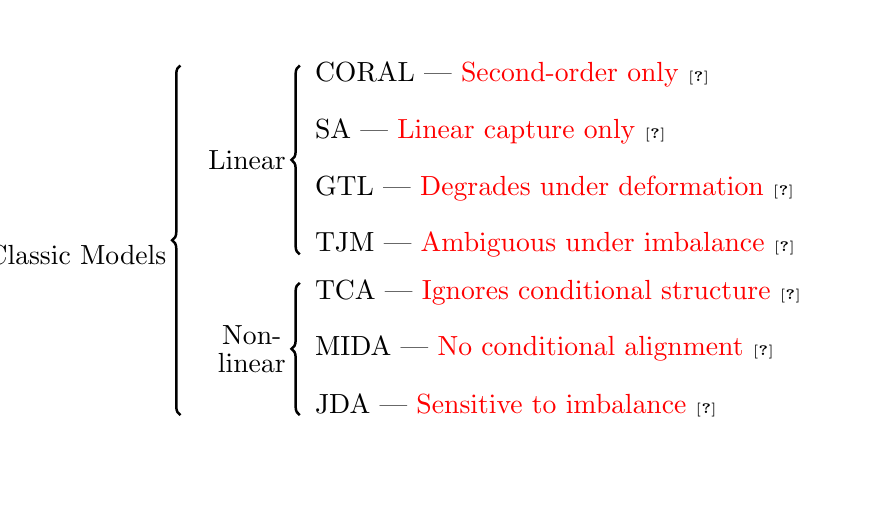
\begin{tikzpicture}[x=\linewidth,y=1.2cm,line width=0.9pt,font=\normalsize]

% ===== styles =====
\tikzset{
  brace/.style={
    draw=none,
    postaction={draw,decorate,decoration={brace,mirror,raise=0pt,amplitude=\amp}}
  },
  lab/.style={anchor=east,fill=white,inner sep=1.2pt}
}

% ===== parameters =====
\path[use as bounding box] (0.14,-2.4) rectangle (1,2.4);

\pgfmathsetmacro{\xMain}{0.30}
\pgfmathsetmacro{\xInner}{0.425}
\pgfmathsetmacro{\xText}{0.43}

\def\labelpad{0.01}
\def\topbot{0.10}
\def\dy{0.60}          % slightly tighter spacing to fit 4 linear items
\def\yA{1.0}
\def\yB{-1.0}
\def\amp{3pt}

% ===== labels =====
\def\Main{Classic Models}
\def\A{Linear}
\def\B{\shortstack{Non-\\linear}}

% ===== items with short limitations =====
\def\Aone{CORAL --- \textcolor{red}{Second-order only}~\cite{wang2018visual}}
\def\Atwo{SA --- \textcolor{red}{Linear capture only}~\cite{zhang2017joint}}
\def\Athree{GTL --- \textcolor{red}{Degrades under deformation}~\cite{satou2025geometrically}}
\def\Afour{TJM --- \textcolor{red}{Ambiguous under imbalance}~\cite{liang2024adaptive}}

\def\Bone{TCA --- \textcolor{red}{Ignores conditional structure}~\cite{yan2017learning}}
\def\Btwo{MIDA --- \textcolor{red}{No conditional alignment}~\cite{leon2020joint}}
\def\Bthree{JDA --- \textcolor{red}{Sensitive to imbalance}~\cite{chen2025deep}}

% ===== main braces =====
\draw[brace] (\xMain,\yA+1.5*\dy+\topbot) -- (\xMain,\yB-\dy-\topbot);
\node[lab] at (\xMain-\labelpad,0) {\Main};

% Linear group brace spans 4 items (±1.5*dy)
\draw[brace] (\xInner,\yA+1.5*\dy+\topbot) -- (\xInner,\yA-1.5*\dy-\topbot);
\node[lab] at (\xInner-\labelpad,\yA) {\A};

% Non-linear group brace unchanged (3 items, ±dy)
\draw[brace] (\xInner,\yB+\dy+\topbot) -- (\xInner,\yB-\dy-\topbot);
\node[lab] at (\xInner-\labelpad,\yB) {\B};

% ===== item nodes =====
% Linear (4 items, centered around yA)
\node[anchor=west] at (\xText,\yA+1.5*\dy) {\Aone};
\node[anchor=west] at (\xText,\yA+0.5*\dy) {\Atwo};
\node[anchor=west] at (\xText,\yA-0.5*\dy) {\Athree};
\node[anchor=west] at (\xText,\yA-1.5*\dy) {\Afour};

% Non-linear (3 items)
\node[anchor=west] at (\xText,\yB+\dy) {\Bone};
\node[anchor=west] at (\xText,\yB)     {\Btwo};
\node[anchor=west] at (\xText,\yB-\dy) {\Bthree};

\end{tikzpicture}
\vspace{-1em}
\end{figure}
\begin{center}
    \textcolor{blue}{Classical methods face robustness limits under heterogeneous domain shifts~\cite{mahmoodiyan2025feature}}
\end{center}

\end{frame}

\begin{frame}{Deep Models for Domain Invariance}
  
    % --- Bloques de contenido ---
    \begin{columns}[T]
    \footnotesize
        % --- Columna Izquierda: Adversarial Invariance ---
        \begin{column}{0.48\textwidth}
            \begin{block}{Domain-Adversarial Neural Network(DANN)}
                \begin{minipage}{\linewidth}
                \begin{align*}
                    \vphantom{\sum_{l}}
                    \min_{\mathcal{F}, \mathcal{G}} \max_{\tilde{\mathcal{G}}} \; & \mathcal{L}_{\mathrm{sup}}(\mathcal{G}(\mathcal{F}(\ve{X}_s)), \ve{y}_s) \;+\;\lambda\; \mathcal{L}_{\mathrm{ad}}(\tilde{\mathcal{G}}(\mathcal{F}(\ve{X})))
                \end{align*}
                \end{minipage}
            \end{block}
        \end{column}
        
        \hfill % Separador
        
        % --- Columna Derecha: Direct Discrepancy Minimization ---
        \begin{column}{0.48\textwidth}
            \begin{block}{Statistical Discrepancy Minimization}
                \begin{minipage}{\linewidth}
                \begin{align*}
                    \min_{\mathcal{F}, \mathcal{G}}\; & \mathcal{L}_{\mathrm{sup}}(\mathcal{G}(\mathcal{F}(\ve{X}_s)), \ve{y}_s) \;+\;\lambda\,\sum_{l}^L \mathcal{L}_{\mathrm{stat}}\bigl(f_l(\ve{X}_s),f_l(\ve{X}_t)\bigr)
                \end{align*}
                \end{minipage}
            \end{block}
        \end{column}
    \end{columns}

    % --- Definiciones al final (solo notación matemática) ---
    \vspace{1cm} 
    \footnotesize 
    $\mat{X}_t \in \mathbb{R}^{n_t \times d}$, $\ve{y}_s\in \mathbb{R}^{n_s}$, $\mathcal{F}: \mathbb{R}^{d} \to \mathbb{R}^{d'}$, $\mathcal{G}: \mathbb{R}^{d'} \to [0,1]^C$, $\tilde{\mathcal{G}}: \mathbb{R}^{d'} \to [0,1]$, $f_l(\cdot)$ stands for the $l$-th feature extractor layer {($ l\in\{1,\dots,L\}$)} , $\lambda \in \mathbb{R}^+$

\end{frame}
% \begin{frame}{Deep Models for Domain Invariance}
%     \vspace{-2cm}
%     Given source $\mathcal{D}^s = \{(\ve{x}_i^s, \ve{y}_i^s)\}_{i=1}^{n_s}$ and target $\mathcal{D}^t = \{\ve{x}_j^t\}_{j=1}^{n_t}$ domains over $\mathcal{X} \subseteq \mathbb{R}^p$, with $\ve{X} = \ve{X}_s \cup \ve{X}_t$.
%     Let $\mathcal{F}: \mathcal{X} \to \mathbb{R}^{d'}$ be a feature extractor composed of $L$ layers, where $f_l(\cdot)$ is the $l$-th layer's output for $l \in \{1, \dots, L\}$.
%     Let $\mathcal{C}: \mathbb{R}^{d'} \to [0,1]^C$ be a classifier and $\mathcal{G}: \mathbb{R}^{d'} \to [0,1]$ a domain discriminator.
%     Let $\lambda, \alpha \in \mathbb{R}^+$ be trade-off hyperparameters.

%     \begin{columns}[T]
%     \footnotesize
%         % --- Left Column: Adversarial Invariance ---
%         \begin{column}{0.5\textwidth}
%             \textbf{Domain-Adversarial NN (DANN)}
%             \begin{align*}
%             \min_{\mathcal{F}, \mathcal{C}} \max_{\mathcal{G}} \; & \mathcal{L}_{\mathrm{sup}}(\mathcal{C}(\mathcal{F}(\ve{X}_s)), \ve{y}_s) \;+\;\lambda\; \mathcal{L}_{\mathrm{ad}}(\mathcal{G}(\mathcal{F}(\ve{X})))
%             \end{align*}
%         \end{column}
        
%         % --- Right Column: Direct Discrepancy Minimization ---
%         \begin{column}{0.5\textwidth}
%             \textbf{Statistical Discrepancy Minimization}
%             \begin{align*}
%             \min_{\mathcal{F}, \mathcal{C}}\; & \mathcal{L}_{\mathrm{sup}}(\mathcal{C}(\mathcal{F}(\ve{X}_s)), \ve{y}_s) \;+\;\alpha\,\sum_{l} \mathcal{L}_{\mathrm{stat}}\bigl(f_l(\ve{X}_s),f_l(\ve{X}_t)\bigr)
%             \end{align*}
%         \end{column}
%     \end{columns}

% \end{frame}







\begin{frame}{Preservation of Domain-Invariant Features}

\begin{figure}
\centering
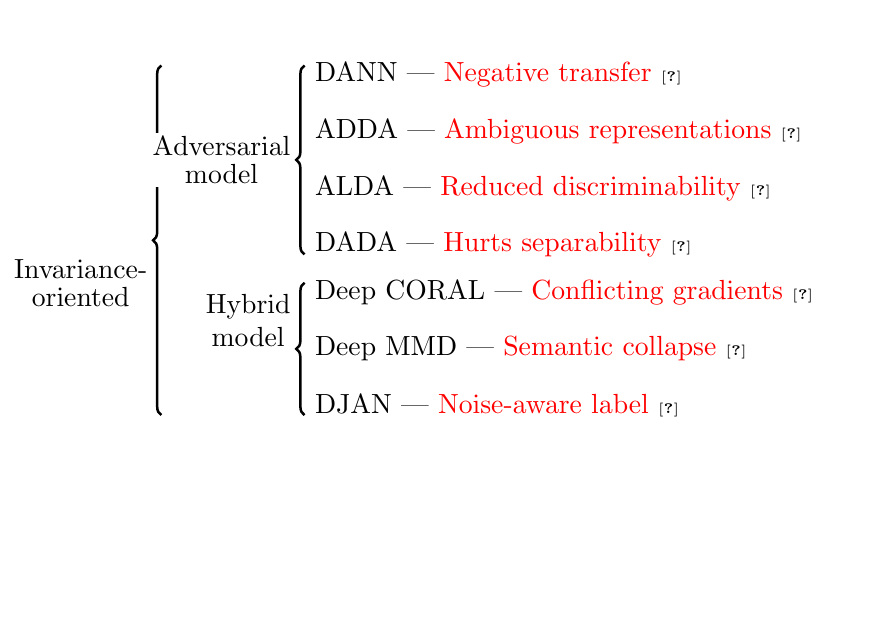
\begin{tikzpicture}[x=\linewidth,y=1.2cm,line width=0.9pt,font=\normalsize]

% ===== styles =====
\tikzset{
  brace/.style={
    draw=none,
    postaction={draw,decorate,decoration={brace,mirror,raise=0pt,amplitude=\amp}}
  },
  lab/.style={anchor=east,fill=white,inner sep=1.2pt}
}

% ===== parameters =====
\path[use as bounding box] (0.14,-3.0) rectangle (1,3.0);

\pgfmathsetmacro{\xMain}{0.28}
\pgfmathsetmacro{\xInner}{0.43}
\pgfmathsetmacro{\xText}{0.43}

\def\labelpad{0.01}
\def\topbot{0.10}
\def\dy{0.6}
\def\amp{3pt}

% vertical anchors por subgrupos
\def\yA{1.6}   % Adversarial invariance (4 ítems)
\def\yB{-0.1}   % Statistical alignment (2 ítems)
\def\yC{-1.2}  % Hybrid joint alignment (1 ítem)

% ===== labels =====
\def\Main{\shortstack{Invariance-\\oriented}}
\def\A{\shortstack{Adversarial\\model}}
\def\B{\shortstack{Hybrid\\model}}

% ===== items =====
% A (4)
\def\Aone{DANN --- \textcolor{red}{Negative transfer}~\cite{mehra2021understanding}}
\def\Atwo{ADDA --- \textcolor{red}{Ambiguous representations}~\cite{gao2023adda}}
\def\Athree{ALDA --- \textcolor{red}{Reduced discriminability}~\cite{kalina2023improving}}
\def\Afour{DADA --- \textcolor{red}{Hurts separability}~\cite{chen2022reusing}}

% B (2)
\def\Bone{Deep CORAL --- \textcolor{red}{Conflicting gradients}~\cite{wang2021p}}
\def\Btwo{Deep MMD --- \textcolor{red}{Semantic collapse}~\cite{zhao2022new}}
\def\Bthree{DJAN --- \textcolor{red}{Noise-aware label}~\cite{li2025multi}}
% C (1)

% ===== main brace =====
\draw[brace] (\xMain,\yA+1.5*\dy+\topbot) -- (\xMain,\yB-1.5*\dy-\topbot);
\node[lab] at (\xMain-\labelpad,0.3) {\Main};

% ===== subgroup braces =====
% A: 4 ítems (±1.5*dy)
\draw[brace] (\xInner,\yA+1.5*\dy+\topbot) -- (\xInner,\yA-1.5*\dy-\topbot);
\node[lab] at (\xInner-\labelpad,\yA) {\A};

% B: 2 ítems (±0.5*dy)
\draw[brace] (\xInner,\yB+0.5*\dy+\topbot) -- (\xInner,\yB-1.5*\dy-\topbot);
\node[lab] at (\xInner-\labelpad,\yB) {\B};



% ===== item nodes =====
% A (4)
\node[anchor=west] at (\xText,\yA+1.5*\dy) {\Aone};
\node[anchor=west] at (\xText,\yA+0.5*\dy) {\Atwo};
\node[anchor=west] at (\xText,\yA-0.5*\dy) {\Athree};
\node[anchor=west] at (\xText,\yA-1.5*\dy) {\Afour};

% B (2)
\node[anchor=west] at (\xText,\yB+0.5*\dy) {\Bone};
\node[anchor=west] at (\xText,\yB-0.5*\dy) {\Btwo};
\node[anchor=west] at (\xText,\yB-1.5*\dy) {\Bthree};
% C (1)

\end{tikzpicture}
\vspace{-4em}
\end{figure}
\begin{center}
\textcolor{blue}{Domain-invariance alignment harms separability, inducing negative transfer \cite{chen2022reusing}.}\\    
\end{center}

\end{frame}

\begin{frame}{Deep Models for Discriminability Preservation}
    \begin{columns}[T]
    \footnotesize
        % --- Columna Izquierda: Knowledge Transfer ---
        \begin{column}{0.38\textwidth}
            \begin{block}{Teacher-Student Framework}
                % Forzamos el ancho con minipage
                \begin{minipage}{\linewidth}
                \begin{align*}
                    \text{1. Teacher: } & \quad \hat{\ve{y}}_t = \arg\max \mathcal{G}_{Te}(\mathcal{F}_{Te}(\ve{X}_t)) \\[.5em]
                    \text{2. Student: }   & \quad \min_{\mathcal{F}_{St}, \mathcal{G}_{St}} \mathcal{L}_{\mathrm{sup}}(\mathcal{G}_{St}(\mathcal{F}_{St}(\ve{X}_t)), \hat{\ve{y}}_t)
                \end{align*}
                \end{minipage}
            \end{block}
        \end{column}
        
        \hfill % Separador
        
        % --- Columna Derecha: Conditional Adversarial Alignment ---
        \begin{column}{0.58\textwidth}
    \begin{block}{Conditional DANN (CDAN)}
        % Forzamos el ancho con minipage
        \begin{minipage}{\linewidth}
        \begin{align*}
            \min_{\mathcal{F}, \mathcal{G}} \max_{\tilde{\mathcal{G}}} \; & \mathcal{L}_{\mathrm{sup}}(\mathcal{G}(\mathcal{F}(\ve{X}_s)), \ve{y}_s) - \lambda\; \mathcal{L}_{\mathrm{adv}}\left(\tilde{\mathcal{G}}(\mathcal{F}(\mat{X}) \otimes \mathcal{G}(\mathcal{F}(\mat{X})))\right)
        \end{align*}
        % \vfill añade espacio vertical si es necesario
        \vfill 
        \end{minipage}
    \end{block}
\end{column}
    \end{columns}

    % --- Definiciones al final (solo notación matemática) ---
    \vspace{1cm}
    \footnotesize
    With $\hat{\ve{y}}_t \text{ (pseudo-labels)}$, $Te, St \text{ (Teacher, Student)}$, $\otimes \text{ (multilinear map)}$

\end{frame}


% \begin{frame}{Deep Models for Discriminability Preservation}
%     \vspace{-2cm}
%     Let $\ve{f} = \mathcal{F}(\ve{x}) \in \mathbb{R}^{d'}$ be the feature vector and $\hat{\ve{g}} = \mathcal{C}(\ve{f}) \in [0,1]^C$ the posterior probability vector. $T$ and $S$ denote the Teacher and Student models, and $\hat{\ve{y}}_t$ are the pseudo-labels for $\mathcal{D}^t$.
%     For CDAN, let $\gamma \in \mathbb{R}^+$ be a trade-off hyperparameter and $\otimes$ a multilinear map.
    
%     \begin{columns}[T]
%     \footnotesize
%         % --- Left Column: Knowledge Transfer via Pseudo-Labels ---
%         \begin{column}{0.5\textwidth}
%             \textbf{Teacher-Student Framework}
%             \begin{align*}
%             \text{1. Teacher: } & \quad \hat{\ve{y}}_t = \arg\max \mathcal{C}_T(\mathcal{F}_T(\ve{X}_t)) \\[.5em]
%             \text{2. Student: }   & \quad \min_{\mathcal{F}_S, \mathcal{C}_S} \mathcal{L}_{\mathrm{sup}}(\mathcal{C}_S(\mathcal{F}_S(\ve{X}_t)), \hat{\ve{y}}_t)
%             \end{align*}
%         \end{column}
        
%         % --- Right Column: Conditional Adversarial Alignment ---
%         \begin{column}{0.5\textwidth}
%             \textbf{Conditional DANN (CDAN)}
%             \begin{align*}
%             \min_{\mathcal{F}, \mathcal{C}} \max_{\mathcal{g}} \; & \mathcal{L}_{\mathrm{sup}}(\mathcal{C}(\mathcal{F}(\ve{X}_s)), \ve{y}_s) 
%             \;+\;\gamma\; \mathcal{L}_{\mathrm{c\text{-}ad}}\left(\ve{f} \otimes \hat{\ve{g}}\right)
%             \end{align*}
%         \end{column}
%     \end{columns}
% \end{frame}


\begin{frame}{Maintenance of Discriminative Features \#1}

\begin{figure}
\centering
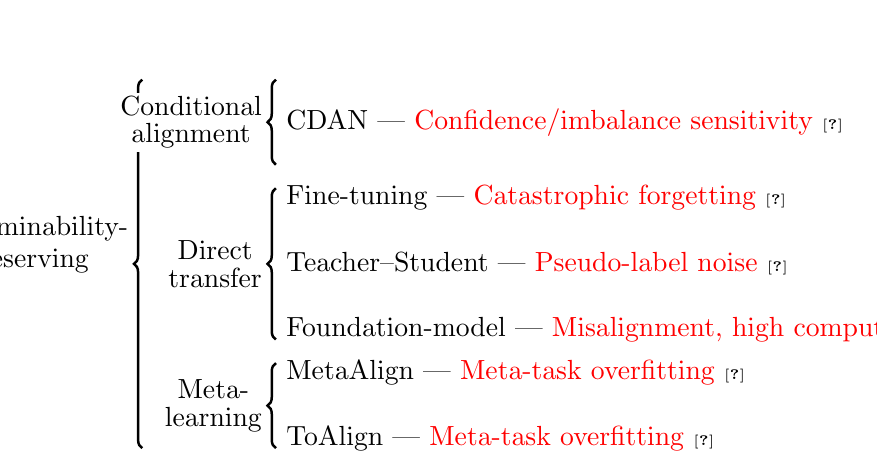
\begin{tikzpicture}[x=\linewidth,y=1.2cm,line width=0.9pt,font=\normalsize]

% ===== styles =====
\tikzset{
  brace/.style={
    draw=none,
    postaction={draw,decorate,decoration={brace,mirror,raise=0pt,amplitude=\amp}}
  },
  lab/.style={anchor=east,fill=white,inner sep=1.2pt}
}

% ===== parameters =====
\path[use as bounding box] (0.14,-0.4) rectangle (1,3.8);

\pgfmathsetmacro{\xMain}{0.26}
\pgfmathsetmacro{\xInner}{0.40}
\pgfmathsetmacro{\xText}{0.40}

\def\labelpad{0.01}
\def\topbot{0.10}
\def\dy{0.70}
\def\amp{3pt}

% vertical anchors por subgrupos (solo A, B, C)
\def\yA{2.8}   % Conditional alignment (1)
\def\yB{1.3}   % Direct transfer (3)
\def\yC{-0.2}   % Meta-learning (2)

% ===== labels =====
\def\Main{\shortstack{Discriminability-\\preserving}}
\def\A{\shortstack{Conditional\\alignment}}
\def\B{\shortstack{Direct\\transfer}}
\def\C{\shortstack{Meta-\\learning}}

% ===== items =====
% A (1)
\def\Aone{CDAN --- \textcolor{red}{Confidence/imbalance sensitivity}~\cite{chen2022reusing}}

% B (3)
\def\Bone{Fine-tuning --- \textcolor{red}{Catastrophic forgetting}~\cite{kumar2022fine}}
\def\Btwo{Teacher--Student --- \textcolor{red}{Pseudo-label noise}~\cite{liu2025mutual}}
\def\Bthree{Foundation-model --- \textcolor{red}{Misalignment, high computational}~\cite{chen2024overview}}

% C (2)
\def\Cone{MetaAlign --- \textcolor{red}{Meta-task overfitting}~\cite{li2025hierarchical}}
\def\Ctwo{ToAlign --- \textcolor{red}{Meta-task overfitting}~\cite{li2025hierarchical}}

% ===== main brace =====
\draw[brace] (\xMain,\yA+0.5*\dy+\topbot) -- (\xMain,\yC-0.5*\dy-\topbot);
\node[lab] at (\xMain-\labelpad,1.5) {\Main};

% ===== subgroup braces =====
% A: 1 ítem
\draw[brace] (\xInner,\yA+0.5*\dy+\topbot) -- (\xInner,\yA-0.5*\dy-\topbot);
\node[lab] at (\xInner-\labelpad,\yA) {\A};

% B: 3 ítems (±dy)
\draw[brace] (\xInner,\yB+\dy+\topbot) -- (\xInner,\yB-\dy-\topbot);
\node[lab] at (\xInner-\labelpad,\yB) {\B};

% C: 2 ítems (±0.5*dy)
\draw[brace] (\xInner,\yC+0.5*\dy+\topbot) -- (\xInner,\yC-0.5*\dy-\topbot);
\node[lab] at (\xInner-\labelpad,\yC) {\C};

% ===== item nodes =====
% A (1)
\node[anchor=west] at (\xText,\yA) {\Aone};

% B (3)
\node[anchor=west] at (\xText,\yB+\dy) {\Bone};
\node[anchor=west] at (\xText,\yB)     {\Btwo};
\node[anchor=west] at (\xText,\yB-\dy) {\Bthree};

% C (2)
\node[anchor=west] at (\xText,\yC+0.5*\dy) {\Cone};
\node[anchor=west] at (\xText,\yC-0.5*\dy) {\Ctwo};

\end{tikzpicture}
\vspace{2.0em}
\end{figure}

\begin{center}
\textcolor{blue}{Discriminative preservation methods often fail due to forgetting and overfitting \cite{kumar2022fine}.}
\end{center}

\end{frame}


\begin{frame}{Maintenance of Discriminative Features \#2}

\begin{figure}
\centering
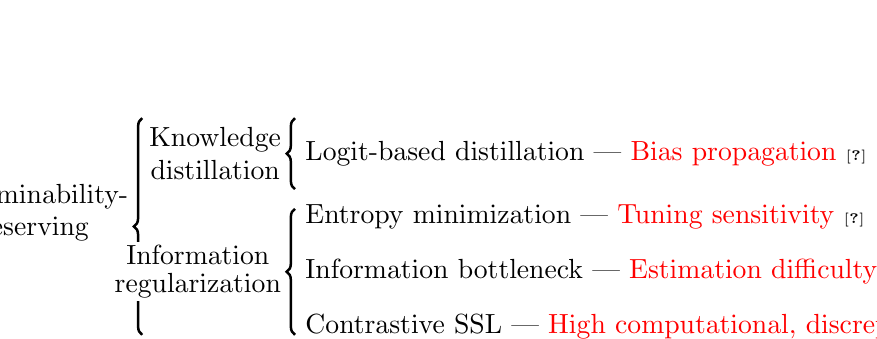
\begin{tikzpicture}[x=\linewidth,y=1.0cm,line width=0.9pt,font=\normalsize]

% ===== styles =====
\tikzset{
  brace/.style={
    draw=none,
    postaction={draw,decorate,decoration={brace,mirror,raise=0pt,amplitude=\amp}}
  },
  lab/.style={anchor=east,fill=white,inner sep=1.2pt}
}

% ===== parameters =====
\path[use as bounding box] (0.14,-1.8) rectangle (1,1.8);

\pgfmathsetmacro{\xMain}{0.26}
\pgfmathsetmacro{\xInner}{0.42}
\pgfmathsetmacro{\xText}{0.42}

\def\labelpad{0.01}
\def\topbot{0.10}
\def\dy{0.70}
\def\amp{3pt}

% vertical anchors por subgrupos (solo D, E)
\def\yD{0.2}   % Knowledge distillation (1)
\def\yE{-1.3}  % Information regularization (3)

% ===== labels =====
\def\Main{\shortstack{Discriminability-\\preserving}}
\def\D{\shortstack{Knowledge\\distillation}}
\def\E{\shortstack{Information\\regularization}}

% ===== items =====
% D (1)
\def\Done{Logit-based distillation --- \textcolor{red}{Bias propagation}~\cite{xing2024hierarchical}}

% E (3)
\def\Eone{Entropy minimization --- \textcolor{red}{Tuning sensitivity}~\cite{poole2019variational}}
\def\Etwo{Information bottleneck --- \textcolor{red}{Estimation difficulty}~\cite{poole2019variational}}
\def\Ethree{Contrastive SSL --- \textcolor{red}{High computational, discrepancies}~\cite{chen2024overview}}

% ===== main brace =====
\draw[brace] (\xMain,\yD+0.5*\dy+\topbot) -- (\xMain,\yE-\dy-\topbot);
\node[lab] at (\xMain-\labelpad,-0.55) {\Main};

% ===== subgroup braces =====
% D: 1 ítem
\draw[brace] (\xInner,\yD+0.5*\dy+\topbot) -- (\xInner,\yD-0.5*\dy-\topbot);
\node[lab] at (\xInner-\labelpad,\yD) {\D};

% E: 3 ítems (±dy)
\draw[brace] (\xInner,\yE+\dy+\topbot) -- (\xInner,\yE-\dy-\topbot);
\node[lab] at (\xInner-\labelpad,\yE) {\E};

% ===== item nodes =====
% D (1)
\node[anchor=west] at (\xText,\yD) {\Done};

% E (3)
\node[anchor=west] at (\xText,\yE+\dy) {\Eone};
\node[anchor=west] at (\xText,\yE)     {\Etwo};
\node[anchor=west] at (\xText,\yE-\dy) {\Ethree};

\end{tikzpicture}
\vspace{5.0em}
\end{figure}

\begin{center}
\textcolor{blue}{Regularization and distillation approaches remain limited by bias propagation \cite{xing2024hierarchical}.}
\end{center}

\end{frame}





\begin{frame}{Interpretability Approaches}

\begin{figure}
\centering
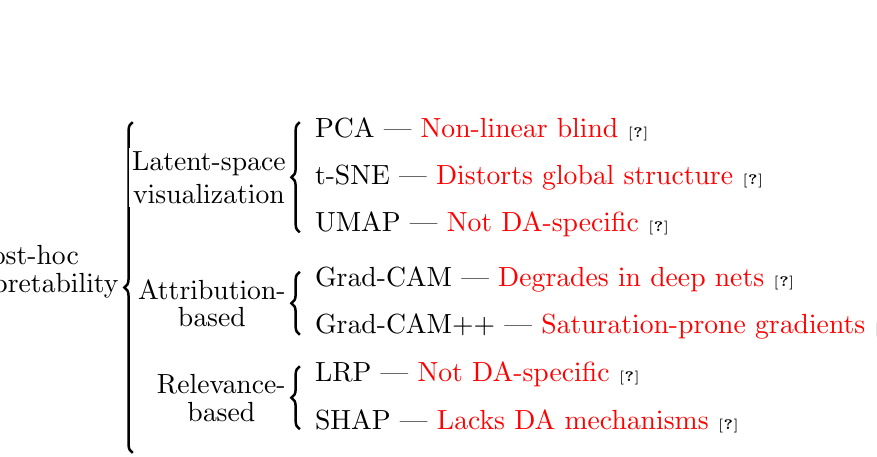
\begin{tikzpicture}[x=\linewidth,y=1.0cm,line width=0.9pt,font=\normalsize]

% ===== styles =====
\tikzset{
  brace/.style={
    draw=none,
    postaction={draw,decorate,decoration={brace,mirror,raise=0pt,amplitude=\amp}}
  },
  lab/.style={anchor=east,fill=white,inner sep=1.2pt}
}

% ===== parameters =====
\path[use as bounding box] (0.14,-2.4) rectangle (1,2.7);

\pgfmathsetmacro{\xMain}{0.25}
\pgfmathsetmacro{\xInner}{0.425}
\pgfmathsetmacro{\xText}{0.43}

\def\labelpad{0.01}
\def\topbot{0.10}
\def\dy{0.60}
\def\amp{3pt}

% vertical anchors por subgrupos
\def\yA{0.8}   % Latent-space visualization (3)
\def\yB{-0.8}   % Attribution-based (2)
\def\yC{-2.0}  % Relevance-based (2)

% ===== labels =====
\def\Main{\shortstack{Post-hoc\\Interpretability}}
\def\A{\shortstack{Latent-space\\visualization}}
\def\B{\shortstack{Attribution-\\based}}
\def\C{\shortstack{Relevance-\\based}}

% ===== items =====
% A (3)
\def\Aone{PCA --- \textcolor{red}{Non-linear blind}~\cite{mirkes2022domain}}
\def\Atwo{t\text{-}SNE --- \textcolor{red}{Distorts global structure}~\cite{jeon2025stop}}
\def\Athree{UMAP --- \textcolor{red}{Not DA-specific}~\cite{ding2025leveraging}}

% B (2)
\def\Bone{Grad\text{-}CAM --- \textcolor{red}{Degrades in deep nets}~\cite{santos2025grad}}
\def\Btwo{Grad\text{-}CAM++ --- \textcolor{red}{Saturation-prone gradients}~\cite{langbein2025gradient}}

% C (2)
\def\Cone{LRP --- \textcolor{red}{Not DA-specific}~\cite{ding2025leveraging}}
\def\Ctwo{SHAP --- \textcolor{red}{Lacks DA mechanisms}~\cite{ding2025leveraging}}

% ===== main brace =====
\draw[brace] (\xMain,\yA+\dy+\topbot) -- (\xMain,\yC-\dy-\topbot);
\node[lab] at (\xMain-\labelpad,-0.4) {\Main};

% ===== subgroup braces =====
% A: 3 ítems (±dy)
\draw[brace] (\xInner,\yA+\dy+\topbot) -- (\xInner,\yA-\dy-\topbot);
\node[lab] at (\xInner-\labelpad,\yA) {\A};

% B: 2 ítems (±0.5*dy)
\draw[brace] (\xInner,\yB+0.5*\dy+\topbot) -- (\xInner,\yB-0.5*\dy-\topbot);
\node[lab] at (\xInner-\labelpad,\yB) {\B};

% C: 2 ítems (±0.5*dy)
\draw[brace] (\xInner,\yC+0.5*\dy+\topbot) -- (\xInner,\yC-0.5*\dy-\topbot);
\node[lab] at (\xInner-\labelpad,\yC) {\C};

% ===== item nodes =====
% A (3)
\node[anchor=west] at (\xText,\yA+\dy) {\Aone};
\node[anchor=west] at (\xText,\yA)     {\Atwo};
\node[anchor=west] at (\xText,\yA-\dy) {\Athree};

% B (2)
\node[anchor=west] at (\xText,\yB+0.5*\dy) {\Bone};
\node[anchor=west] at (\xText,\yB-0.5*\dy) {\Btwo};

% C (2)
\node[anchor=west] at (\xText,\yC+0.5*\dy) {\Cone};
\node[anchor=west] at (\xText,\yC-0.5*\dy) {\Ctwo};

\end{tikzpicture}
\vspace{2.0em}
\end{figure}

\begin{center}
\textcolor{blue}{Lack of adaptation-specific interpretability hinders safe and transparent application \cite{ding2025leveraging}.
}
\end{center}
\end{frame}
    



\section{Aims}

\begin{frame}{General Aim}

   \begin{itemize}
\justifying
   \item Develop a \textbf{deep learning–based} \textbf{DA} framework for \textbf{classification}. It should improve \textbf{generalization}, \textbf{class discrimination}, and \textbf{interpretability} under \textbf{overlapping labels}, \textbf{noisy data}, and \textbf{limited supervision}, while ensuring \textbf{stable} and \textbf{traceable} behavior in \textbf{unseen domains}.

   \end{itemize}
\end{frame}



\begin{frame}{Specific Aims}
   \begin{itemize}
    \setlength\itemsep{2em}
\justifying
     \item[1] Develop a \textbf{regularization mechanism} to enhance model \textbf{robustness} against \textbf{target domain uncertainty}, considering the effect of \textbf{overlapping labels} and \textbf{noisy pseudo-labels} in \textbf{limited supervision} settings.
     
     \item[2] Design an \textbf{alignment strategy} that preserves \textbf{semantic consistency} across domains, in order to reduce the \textbf{class-level distributional discrepancy} and retain \textbf{discriminative information} in the presence of \textbf{covariate shift}.
     
     \item[3] Establish an \textbf{interpretability approach} to facilitate the analysis of the \textbf{semantic coherence} of representations, through the \textbf{qualitative evaluation} of activated regions and their correspondence with \textbf{relevant attributes}, in scenarios characterized by \textbf{high inter-class ambiguity} and \textbf{inter-domain variability}.
    
   \end{itemize}   
\end{frame}

\section{Methodology}


\begin{frame}{Proposal Obj. 1 - 3: Conditional Rényi $\alpha$-Entropy DA - CREDA}

% \begin{figure}
%     \centering \includegraphics[width=0.8\linewidth]{Figures/dibujo_GCCE_bloques_no matth2.pdf}
% \end{figure}

\begin{figure}
    \centering \rasterpdffile[240]{Figures/Met.pdf}{\linewidth}

\end{figure}

% \begin{itemize}
%   \item \textbf{Deep Feature Extraction}: Shared \textbf{feature extractor model} encodes source and target into a \textbf{latent space}.
%   \item \textbf{Noise-Aware Label Weighting}: \textbf{Entropy-based confidence} down-weights low-confidence \textbf{pseudo-labels}.
%   \item \textbf{Class-Conditional Alignment}: \textbf{Rényi entropy regularization} minimizes divergence across \textbf{class-wise distributions}.
% \end{itemize}
\begin{center}
    \textcolor{blue}{CREDA preserves invariance, enforces class alignment, and mitigates noisy pseudo-label effects.}
\end{center}


\end{frame}

% ===================== Materials and Methods =====================

% ---------- Kernel Methods Fundamentals #1 ----------
% ===================== Kernel Methods Fundamentals #1 =====================
% \begin{frame}{Kernel Methods Fundamentals \#1}

% Input space $\mathcal{X}\subseteq\mathbb{R}^d$; RKHS $(\mathcal{H}_\kappa,\langle\cdot,\cdot\rangle_{\mathcal{H}_\kappa})$;
% feature map $\Phi:\mathcal{X}\to\mathcal{H}_\kappa$.
% \emph{Gaussian (RBF) kernel} with bandwidth $\sigma\in\mathbb{R}^+$:
% \[
% \kappa_\sigma(x_i,x_j):=\exp\!\Big(-\tfrac{\|x_i-x_j\|_2^2}{2\sigma^2}\Big).
% \]
% For a sample $\{x_i\}_{i=1}^N$, Gram $\mathbf{K}\in\mathbb{R}^{N\times N}$ with $\mathbf{K}_{ij}=\kappa_\sigma(x_i,x_j)$.

% \medskip
% By the kernel trick,
% \[
% \big\langle \Phi(x_i),\Phi(x_j)\big\rangle_{\mathcal{H}_\kappa}=\kappa_\sigma(x_i,x_j),\quad
% \|\Phi(x)\|_{\mathcal{H}_\kappa}^{2}=\kappa_\sigma(x,x).
% \]


% \medskip
% References:~\cite{scholkopf2018learning,murphy2022probabilistic,wilson2013gaussian}
% \end{frame}



\begin{frame}{Kernel-Based $\alpha$-Rényi's Entropy Estimation \#1}

Continuous $X$ with PDF $f$ on $\chi$; Rényi entropy
\[
H_{\alpha}(X)=\frac{1}{1-\alpha}\log\!\int_{\chi} f(x)^{\alpha}\,dx,\quad \alpha>0,\ \alpha\neq 1.
\]
Kernel density estimate (KDE) with $N$ samples $\{x_i\}_{i=1}^{N}$:
\[
\hat f(x)=\frac{1}{N}\sum_{i=1}^{N}\kappa_\sigma(x,x_i).
\]

\medskip
\textbf{Information Potential (IP), $\alpha=2$.}
The integral $\int f(x)^2dx$ yields (by convolution of Gaussians):
\[
\hat V_2(X)=\int \hat f(x)^2dx
=\frac{1}{N^2}\sum_{i=1}^{N}\sum_{j=1}^{N}\int \kappa_\sigma(x,x_i)\kappa_\sigma(x,x_j)\,dx
=\frac{1}{N^2}\sum_{i,j}\kappa_{\sqrt{2}\sigma}(x_i,x_j)=\frac{1}{N^2}\mathbf{1}^\top \mathbf{K}\,\mathbf{1}.
\]

\footnotesize References: \cite{principe2010information,silverman2018density,bromiley2003products,xu2008reproducing}.
\end{frame}

% ---------- Kernel-Based α-Rényi's Entropy Estimation #2 ----------


\begin{frame}{Kernel-Based $\alpha$-Rényi's Entropy Estimation \#2}

Normalized Gram $\breve{\mathbf{A}}:=\mathbf{K}/\operatorname{tr}(\mathbf{K})$;
Hadamard product $\odot$.

\medskip
\textbf{Matrix-based Rényi entropy.}
\[
H_{\alpha}(\breve{\mathbf{A}})=\frac{1}{1-\alpha}\log\!\big(\operatorname{tr}(\breve{\mathbf{A}}^{\alpha})\big).
\]
For $\alpha=2$ (stable Frobenius form):
\[
H_2(\breve{\mathbf{A}})=-\log\!\big(\operatorname{tr}(\breve{\mathbf{A}}^\top\breve{\mathbf{A}})\big).
\]

\medskip
\textbf{Joint, mutual, and conditional (matrix-based).}
With paired features and Grams $\mathbf{K}_X,\mathbf{K}_Y$:
\[
\mathbf{K}_{XY}:=\mathbf{K}_{X}\odot \mathbf{K}_{Y},\qquad
H_{\alpha}(\mathbf{K}_X,\mathbf{K}_Y)=\frac{1}{1-\alpha}\log\!\big(\operatorname{tr}(\mathbf{K}_{XY}^{\alpha})\big),
\]
\[
I_{\alpha}(\mathbf{K}_X;\mathbf{K}_Y)=H_{\alpha}(\mathbf{K}_X)+H_{\alpha}(\mathbf{K}_Y)-H_{\alpha}(\mathbf{K}_X,\mathbf{K}_Y).
\]
% \[
% H_{\alpha}(\mathbf{K}_X\mid \mathbf{K}_Y)=H_{\alpha}(\mathbf{K}_X,\mathbf{K}_Y)-H_{\alpha}(\mathbf{K}_Y).
% \]

\footnotesize References: \cite{giraldo2014measures,giraldo2013information}.
\end{frame}



\begin{frame}{$\alpha$-Rényi Entropy-Based Label Weighting and Regularization \#1}

Feature extractor $\mathcal{F}:\mathcal{X}\to\mathbb{R}^{d'}$,
classifier $\mathcal{G}:\mathbb{R}^{d'}\to[0,1]^C$ with $\mathbf{g}=\mathcal{G}(\mathbf{f})$.
Source domain $\mathcal{D}^s=\{(\mathbf{x}_i^s,\mathbf{y}_i^s)\}_{i=1}^{N_s}$,
target $\mathcal{D}^t=\{\mathbf{x}_j^t\}_{j=1}^{N_t}$ (unlabeled).
Per-class counts $n_c^s,n_c^t$.

\medskip
\textbf{Class-conditional Gram matrices.}
For each class $c$:
\[
\mathbf{K}_c^s=[\kappa_{\sigma_s}(\mathbf{f}_i^s,\mathbf{f}_{i'}^s)],\quad
\mathbf{K}_c^t=[\kappa_{\sigma_t}(\mathbf{f}_j^t,\mathbf{f}_{j'}^t)],\quad
\mathbf{K}_c^{st}=[\kappa_{\sigma_{st}}(\mathbf{f}_i^s,\mathbf{f}_j^t)],
\]
with $\mathbf{f}_i^s=\mathcal{F}(\mathbf{x}_i^s)$, $\mathbf{f}_j^t=\mathcal{F}(\mathbf{x}_j^t)$,
$y^s_{i,c}=1$, and $\arg\max_{c'} g^t_{j,c'}=c$.

\end{frame}

% ---------- Domain Adaptation with α-Rényi ... #2 ----------
\begin{frame}{$\alpha$-Rényi Entropy-Based Label Weighting and Regularization \#2}

\textbf{Notation (target confidence weights).}
Quadratic Rényi entropy of prediction $g^t_{j,c}\in \mathbf{g}^t_j$, and $\mathbf{g}^t_j=\mathcal{G}(\mathbf{f}_{j}^t)$:
\[
\hat H_2(\mathbf{g}_j^t)=-\log\!\Big(\sum_{c=1}^{C}(g^t_{j,c})^{2}\Big),\quad
\hat U(\mathbf{g}_j^t)=\frac{\hat H_2(\mathbf{g}_j^t)}{\log C}\in[0,1],\quad
w_j^t:=1-\hat U(\mathbf{g}_j^t).
\]

\medskip
\textbf{Weighted target Gram (per class).}
Let $\tilde{\mathbf{w}}_c^t=\{w_j^t:\arg\max_{c'} g^t_{j,c'}=c\}$ and
$\tilde{\mathbf{W}}_c^t:=\tilde{\mathbf{w}}_c^t(\tilde{\mathbf{w}}_c^t)^\top$,
then
\[
\boxed{\;\tilde{\mathbf{K}}_c^t=\mathbf{K}_c^t\odot \tilde{\mathbf{W}}_c^t\;}
\]
down-weights uncertain target pairs while preserving the RKHS geometry (Hadamard reweighting).

\end{frame}

% ---------- Domain Adaptation with α-Rényi ... #3 ----------
\begin{frame}{$\alpha$-Rényi Entropy-Based Label Weighting and Regularization \#3}

\textbf{MI regularizer (per class).}
With the matrix-based $\alpha$-Rényi entropy ($\alpha=2$):
\[
\tilde{\mathrm{I}}_2(\mathbf{K}_c^s;\tilde{\mathbf{K}}_c^t)
=\frac{1}{2}\Big(H_2(\mathbf{K}_c^s)+H_2(\tilde{\mathbf{K}}_c^t)\Big)-H_2(\mathbf{K}_c^{\mathrm{mix}}),
\]
where
\[
\mathbf{K}_c^{\mathrm{mix}}=
\begin{pmatrix}
\mathbf{K}_c^s & \mathbf{K}_c^{st}\\
(\mathbf{K}_c^{st})^\top & \tilde{\mathbf{K}}_c^t
\end{pmatrix}
\]
explicitly handles class-imbalanced sample sizes \((n_c^s \neq n_c^t)\) while capturing within- and cross-domain similarities.


\medskip
\textbf{Total loss.}
\[
\boxed{\;\mathcal{L}_{\mathrm{CREDA}}
=\sum_{i=1}^{N_s}\sum_{c=1}^{C} y^s_{i,c}\,\log\!\big(\mathcal{G}(\mathcal{F}(\mathbf{x}_i^s))\big)
-\lambda \sum_{c=1}^{C}\tilde{\mathrm{I}}_2(\mathbf{K}_c^s;\tilde{\mathbf{K}}_c^t)\;}
\]
with $\lambda>0$ controlling alignment strength.

\end{frame}


\section[Experiments]{Experimental Set-Up and Results on Image Data}
\begin{frame}{Training details and main pipeline}
\small
\begin{figure}
\vspace{-0.5cm}
    \centering  \rasterpdffile[240]{Figures/Set-Up.pdf}{\linewidth}
\end{figure}
\begin{center}

    \textcolor{blue}{Proposed CREDA compared with classical domain adaptation models on image datasets.}
\end{center}
\end{frame}
% \begin{frame}{Digits Benchmark}
% \centering
% 
\includegraphics[width=\linewidth]{Figures/digits.pdf}
% \begin{center}
%     \textcolor{blue}{Digits baseline enables domain adaptation evaluation on diverse scene digits~\cite{sankaranarayanan2018generate}.}
% \end{center}
% \end{frame}


% \begin{frame}{ImageCLEF-DA Benchmark}
% \centering
% 
\includegraphics[width=\linewidth]{Figures/imageclef_grid.pdf}

% \begin{center}
%     \textcolor{blue}{Shared object classes across datasets enable domain adaption with ImageCLEF-DA.~\cite{cheng2022foreground},}
% \end{center}
% \end{frame}

% \begin{frame}{Office-31 Benchmark}
% \centering
% 
\includegraphics[width=\linewidth]{Figures/office_grid.pdf}
% \begin{center}
%     \textcolor{blue}{Office-31 benchmark tests adaptation across visually diverse domains classes~\cite{murez2018image}.}
% \end{center}
% \end{frame}


\begin{frame}{ResNet-18 Feature Extractor}
\begin{table}
\begin{tabularx}{\linewidth}{lcccc}
\toprule
\textbf{Layer Name} & \textbf{Type} & \textbf{Input Shape} & \textbf{Output Shape} & \textbf{Param. \#} \\
\midrule
Input & InputLayer & $(3, \breve{H}, \breve{W})$ & $(3, \breve{H}, \breve{W})$ & 0 \\
Conv1 & Conv2D+BN+ReLU & $(3, \breve{H}, \breve{W})$ & $(64, \breve{H}/2, \breve{W}/2)$ & 9408 \\
MaxPool & MaxPooling & $(64, \breve{H}/2, \breve{W}/2)$ & $(64, \breve{H}/4, \breve{W}/4)$ & 0 \\
Layer1 & Residual Block $\times$2 & $(64, \breve{H}/4, \breve{W}/4)$ & $(64, \breve{H}/4, \breve{W}/4)$ & 73,728 \\
Layer2 & Residual Block $\times$2 & $(64, \breve{H}/4, \breve{W}/4)$ & $(128, \breve{H}/8, \breve{W}/8)$ & 230,144 \\
Layer3 & Residual Block $\times$2 & $(128, \breve{H}/8, \breve{W}/8)$ & $(256, \breve{H}/16, \breve{W}/16)$ & 919,040 \\
Layer4 & Residual Block $\times$2 & $(256, \breve{H}/16, \breve{W}/16)$ & $(512, \breve{H}/32, \breve{W}/32)$ & 3,674,112 \\
AvgPool & GlobalAvgPooling & $(512, \breve{H}/32, \breve{W}/32)$ & $(512, 1, 1)$ & 0 \\
Flatten & Flatten & $(512,1,1)$ & $(512)$ & 0 \\
\midrule
\multicolumn{4}{r}{\textbf{Total}} & \textbf{4,906,432} \\
\midrule
\end{tabularx}
\end{table}
\begin{center}
    \textcolor{blue}{ResNet-18 extracts transferable spatial features across domains~\cite{diagnostics11061071}.}
\end{center}
\end{frame}

\begin{frame}{ResNet-50 Feature Extractor}
\begin{table}
\footnotesize
\begin{tabularx}{\linewidth}{p{1.5cm}lcccc}
\toprule
\textbf{Layer Name} & \textbf{Type} & \textbf{Input Shape} & \textbf{Output Shape} & \textbf{Param. \#} \\
\midrule
Input & InputLayer & $(3, \breve{H}, \breve{W})$ & $(3, \breve{H}, \breve{W})$ & 0 \\
Conv1 & Conv2D+BN+ReLU & $(3, \breve{H}, \breve{W})$ & $(64, \breve{H}/2, \breve{W}/2)$ & 9408 \\
MaxPool & MaxPooling & $(64, \breve{H}/2, \breve{W}/2)$ & $(64, \breve{H}/4, \breve{W}/4)$ & 0 \\
Layer1 & Bottleneck Block $\times$3 & $(64, \breve{H}/4, \breve{W}/4)$ & $(256, \breve{H}/4, \breve{W}/4)$ & 214,528 \\
Layer2 & Bottleneck Block $\times$4 & $(256, \breve{H}/4, \breve{W}/4)$ & $(512, \breve{H}/8, \breve{W}/8)$ & 1,182,720 \\
Layer3 & Bottleneck Block $\times$6 & $(512, \breve{H}/8, \breve{W}/8)$ & $(1024, \breve{H}/16, \breve{W}/16)$ & 7,084,032 \\
Layer4 & Bottleneck Block $\times$3 & $(1024, \breve{H}/16, \breve{W}/16)$ & $(2048, \breve{H}/32, \breve{W}/32)$ & 15,085,568 \\
AvgPool & GlobalAvgPooling & $(2048, \breve{H}/32, \breve{W}/32)$ & $(2048, 1, 1)$ & 0 \\
Flatten & Flatten & $(2048,1,1)$ & $(2048)$ & 0 \\
\midrule
\multicolumn{4}{r}{\textbf{Total}} & \textbf{23,576,256} \\
\midrule
\end{tabularx}
\end{table}
\begin{center}
    \textcolor{blue}{ResNet-50 employs bottleneck blocks for deeper feature extraction~\cite{mascarenhas2021comparison}.}
\end{center}
\end{frame}

\begin{frame}{ViT-Tiny Feature Extractor}

\begin{table}
\begin{tabularx}{\linewidth}{lcccc}
\toprule
\textbf{Layer Name} & \textbf{Type} & \textbf{Input Shape} & \textbf{Output Shape} & \textbf{Param. \#} \\
\midrule
Input & InputLayer & $(3,224,224)$ & $(3,224,224)$ & 0 \\
Patch Embedding & Conv2D (Patching) & $(3,224,224)$ & $(196,192)$ & 147,648 \\
Add CLS Token & Concatenation & $(196,192)$ & $(197,192)$ & 192 \\
Add Pos. Embedding & Parameter Add & $(197,192)$ & $(197,192)$ & 37,824 \\
Transformer Encoder & Encoder Block $\times$12 & $(197,192)$ & $(197,192)$ & 5,529,792 \\
Extract CLS Token & Indexing & $(197,192)$ & $(1,192)$ & 0 \\
LayerNorm & LayerNorm & $(1,192)$ & $(1,192)$ & 384 \\
Flatten & Flatten & $(1,192)$ & $(192)$ & 0 \\
\midrule
\multicolumn{4}{r}{\textbf{Total}} & \textbf{5,715,840} \\
\midrule
\end{tabularx}
\end{table}
\begin{center}
    \textcolor{blue}{ViT-Tiny encodes image with  Transformer blocks for learning representations.~\cite{dosovitskiy2020image}.}
\end{center}

\end{frame}
\begin{frame}{Classifier and Discriminator}
\begin{table}
\begin{tabularx}{\linewidth}{lcccc}
\toprule
\textbf{Layer Name} & \textbf{Type} & \textbf{Input Shape} & \textbf{Output Shape} & \textbf{Param. \#} \\
\midrule
Input   & InputLayer  & $(d,)$ & $(d,)$ & 0 \\
FC1     & Dense       & $(d,)$ & $(d/2,)$ & $(d \times d/2)+d/2$ \\
BN1     & BatchNorm1d & $(d/2,)$ & $(d/2,)$ & $d$ \\
ReLU1   & Activation  & $(d/2,)$ & $(d/2,)$ & 0 \\
FC2     & Dense       & $(d/2,)$ & $(d/4,)$ & $(d/2 \times d/4)+d/4$ \\
BN2     & BatchNorm1d & $(d/4,)$ & $(d/4,)$ & $d/2$ \\
ReLU2   & Activation  & $(d/4,)$ & $(d/4,)$ & 0 \\
Output  & Dense       & $(d/4,)$ & $(C \text{ or } 1)$ & $(d/4 \times (C \text{ or } 1))+(C \text{ or } 1)$ \\
\midrule
\multicolumn{4}{r}{\textbf{Total}} & $\frac{5}{8}d^2 + \frac{9}{4}d + (C \text{ or } 1)\left(\frac{d}{4} + 1\right)$ \\
\midrule
\end{tabularx}
\end{table}
\begin{center}
    \textcolor{blue}{Classifier and discriminator share structure; only output layer differs~\cite{ganin2016domain}.}
\end{center}
\end{frame}

\begin{frame}{Method Comparison}

\begin{columns}

\begin{column}{0.5\textwidth} % Columna izquierda: Ecuaciones de los métodos
\tiny
\textbf{Baseline}:
\begin{equation*}
\mathcal{L}_{\text{Baseline}} 
= - \sum_{i=1}^{N_s}\sum_{c=1}^{C} 
y^s_{i,c}\,\log\!\left(\mathcal{G}(\mathcal{F}(\mathbf{x}^s_i))\right).
\label{eq:loss_baseline}
\end{equation*}
\vspace{-0.3cm}
\textbf{DANN}~\cite{jin2025improved}:
\begin{equation*}
\mathcal{L}_{\text{DANN}} 
= \mathcal{L}_{\text{Baseline}} + 
\lambda\!\left[
- \sum_{i=1}^{N_s}\log\!\big(\tilde{\mathcal{G}}(\mathcal{F}(\mathbf{x}^s_i))\big)
- \sum_{j=1}^{N_t}\log\!\big(1-\tilde{\mathcal{G}}(\mathcal{F}(\mathbf{x}^t_j))\big)
\right].
\label{eq:loss_dann_full}
\end{equation*}
\vspace{-0.3cm}
\textbf{ADDA}~\cite{li2025cross}:
\begin{equation*}
\mathcal{L}_{\text{ADDA}} = 
\underbrace{\mathcal{L}_{\text{Baseline}}}_{\text{Stage 1}}
+
\underbrace{\lambda\left[
- \sum_{i=1}^{N_s}\log\!\big(\tilde{\mathcal{G}}(\mathcal{F}^s(\mathbf{x}^s_i))\big)
- \sum_{j=1}^{N_t}\log\!\big(1-\tilde{\mathcal{G}}(\mathcal{F}^t(\mathbf{x}^t_j))\big)
\right]}_{\text{Stage 2}}.
\label{eq:loss_adda_full}
\end{equation*}
\vspace{-0.3cm}
\textbf{CDAN+E}~\cite{deng2025bearing}:
\begin{equation*}
\breve{w}_j = 1 + \exp(-H(\mathcal{G}(\mathcal{F}^t(\mathbf{x}^t_j)))),
\end{equation*}
\vspace{-0.3cm}
\begin{equation*}
\mathcal{L}_{\text{CDAN+E}} 
= \mathcal{L}_{\text{Baseline}} + \lambda\!\left[
- \sum_{i=1}^{N_s} \breve{w}_i^s 
\log\!\big(\tilde{\mathcal{G}}(\mathcal{F}^s(\mathbf{x}^s_i))\big)
- \sum_{j=1}^{N_t} \breve{w}_j^t 
\log\!\big(1-\tilde{\mathcal{G}}( \mathcal{F}^t(\mathbf{x}^t_j))\big)
\right].
\label{eq:loss_cdan_full}
\end{equation*}
\end{column}

\begin{column}{0.5\textwidth} % Columna derecha: Imagen
\centering
\rasterpdffile[240]{Figures/eta_lambda_plot.pdf}{\linewidth}

\end{column}

\end{columns}
\begin{center}
    \textcolor{blue}{Dynamic scheduling shifts from feature learning to stable domain alignment~\cite{deng2025bearing}.}
\end{center}
\end{frame}






\begin{frame}{Statistical Validation — Friedman Test - Obj. 1}
\begin{table}
\footnotesize
%\centering %% If there is a figure in wide page, please release command \centering
\begin{tabularx}{\linewidth}{llccccc}
\toprule
\textbf{Dataset} & \textbf{Backbone} & \textbf{Baseline} & \textbf{DANN} & \textbf{ADDA} & \textbf{CDAN+E} & \textbf{CREDA (Ours)} \\
\midrule
% --- Ranks from Digits Dataset ---
 & ResNet-18 & 4.0 & 2.0 & 3.0 & 5.0 & 1.0 \\
Digits & ResNet-50 & 4.0 & 2.0 & 3.0 & 5.0 & 1.0 \\
 & ViT-Tiny  & 1.0 & 3.0 & 5.0 & 4.0 & 2.0 \\
\midrule
% --- Ranks from ImageCLEF-DA Dataset ---
& ResNet-18 & 4.0 & 3.0 & 2.0 & 5.0 & 1.0 \\
ImageCLEF-DA & ResNet-50 & 4.0 & 1.0 & 3.0 & 5.0 & 2.0 \\
 & ViT-Tiny  & 2.0 & 3.0 & 4.0 & 5.0 & 1.0 \\
\midrule
% --- Ranks from Office-31 Dataset ---
 & ResNet-18 & 5.0 & 2.0 & 3.0 & 4.0 & 1.0 \\
Office-31 & ResNet-50 & 5.0 & 2.0 & 3.0 & 4.0 & 1.0 \\
 & ViT-Tiny  & 2.0 & 4.0 & 3.0 & 5.0 & 1.0 \\
\midrule
\textbf{Mean Rank ± Std%MDPI: Please confirm if the bold formatting is necessary; if not, please remove it. Same as below. Ans: We confirm the bold formatting is necessary
} & -- & 3.4 $\pm$ 1.4 & 2.4 $\pm$ 0.9 & 3.2 $\pm$ 0.8 & 4.7 $\pm$ 0.5 & \textbf{1.2 $\pm$ 0.4} %Ans: We confirm the bold formatting is necessary
\\
\bottomrule
\end{tabularx}
\end{table}
\begin{center}
    \textcolor{blue}{CREDA ranks first with lowest variance, confirming consistent superiority \tiny($\chi^2 = 23.21$, $p < 1.15\times10^{-4} $)}.
\end{center}
\end{frame}




% \begin{frame}{UMAP Across Adaptation Methods - Obj. 3}
% \centering
% \rasterpdffile[240]{Figures/umap_projection.pdf}{0.8\linewidth}
% \begin{center}
%     \textcolor{blue}{CREDA ensures domain alignment while preserving class-wise structure and separability.}
% \end{center}
% \end{frame}




\begin{frame}{Interpretable Visual Explanations - Obj. 3}
\centering
\rasterpdffile[240]{Figures/Cams.pdf}{0.8\linewidth}

\begin{center}
    \textcolor{blue}{CREDA focuses on semantically relevant regions across domains, enhancing trust.}
\end{center}
\end{frame}

\begin{frame}{Computational Efficiency Analysis - Obj. 1-3}
\centering
\rasterpdffile[240]{Figures/CostoC.pdf}{0.6\linewidth}

\begin{center}
    \textcolor{blue}{CREDA balances high accuracy with manageable training cost and fast inference.}
\end{center}
\end{frame}


\section[ ]{Experimental Set-Up and Results on EEG Data}
\begin{frame}{Training details and main pipeline}
\small
\begin{figure}
\vspace{-0.5cm}
    \centering \rasterpdffile[240]{Figures/Set-Up_1.pdf}{\linewidth}
\end{figure}
\begin{center}

    \textcolor{blue}{Proposed CREDA compared with classical domain adaptation models on EEG datasets.}
\end{center}
\end{frame}


% \begin{frame}{GigaScience DB-I Protocol}
% \centering
% \begin{minipage}[c]{0.7\linewidth}
%   
\includegraphics[width=\linewidth]{Figures/GIGA_experiment.jpeg}
% \end{minipage}\hfill
% \begin{minipage}[c]{0.3\linewidth}
%   
\includegraphics[trim={0.9cm 0cm 0cm 0cm},clip,width=\linewidth]{Figures/GIGA_montage.jpeg}
% \end{minipage}

% \vspace{1em}
% {\textcolor{blue}{EEG datasets for motor imagery brain computer interface~\cite{https://doi.org/10.5524/100295}.}}
% \end{frame}

\begin{frame}{EEGNet Feature Extractor}

\begin{table}
\scriptsize
\begin{tabularx}{\linewidth}{p{2.85cm}p{3.5cm}p{2.85cm}p{2.85cm}lcccc}
\toprule
\textbf{Layer Name} & \textbf{Type} & \textbf{Input Shape} & \textbf{Output Shape} & \textbf{Param. \#} \\
\midrule
Input        & InputLayer         & $(1,64,320)$   & $(1,64,320)$   & $0$ \\
TemporalConv & Conv2D             & $(1,64,320)$   & $(32,64,320)$  & $2{,}048$ \\
BN1          & BatchNormalization & $(32,64,320)$  & $(32,64,320)$  & $64$ \\
SpatialConv  & DepthwiseConv2D    & $(32,64,320)$  & $(64,1,320)$   & $4{,}096$ \\
BN2          & BatchNormalization & $(64,1,320)$   & $(64,1,320)$   & $128$ \\
ELU1         & Activation         & $(64,1,320)$   & $(64,1,320)$   & $0$ \\
AvgPool1     & AveragePooling2D   & $(64,1,320)$   & $(64,1,20)$    & $0$ \\
Dropout1     & Dropout            & $(64,1,20)$    & $(64,1,20)$    & $0$ \\
SepConv      & SeparableConv2D    & $(64,1,20)$    & $(64,1,20)$    & $8{,}192$ \\
BN3          & BatchNormalization & $(64,1,20)$    & $(64,1,20)$    & $128$ \\
ELU2         & Activation         & $(64,1,20)$    & $(64,1,20)$    & $0$ \\
AvgPool2     & AveragePooling2D   & $(64,1,20)$    & $(64,1,1)$     & $0$ \\
Dropout2     & Dropout            & $(64,1,1)$     & $(64,1,1)$     & $0$ \\
Flatten      & Flatten            & $(64,1,1)$     & $(64)$         & $0$ \\
\midrule
\multicolumn{4}{r}{\textbf{Total}} & $\mathbf{14{,}656}$ \\
\midrule

\end{tabularx}
\end{table}

\begin{center}
\textcolor{blue}{EEGNet learns compact temporal–spatial EEG representations~\cite{lawhern2018eegnet}.}
\end{center}
\end{frame}

\begin{frame}{ShallowConvNet Feature Extractor}

\begin{table}
\begin{tabularx}{\linewidth}{p{2.6cm}p{3.5cm}p{2.6cm}p{2.8cm}p{2.6cm}lcccc}
\toprule
\textbf{Layer Name} & \textbf{Type} & \textbf{Input Shape} & \textbf{Output Shape} & \textbf{Param. \#} \\
\midrule
Input         & InputLayer         & $(64,320,1)$   & $(1,64,320)$   & $0$ \\
TemporalConv  & Conv2D             & $(1,64,320)$   & $(40,64,308)$  & $560$ \\
SpatialConv   & Conv2D             & $(40,64,308)$  & $(40,1,308)$   & $102{,}440$ \\
BN1           & BatchNormalization & $(40,1,308)$   & $(40,1,308)$   & $80$ \\
Activation1   & Square             & $(40,1,308)$   & $(40,1,308)$   & $0$ \\
AvgPool1      & AveragePooling2D   & $(40,1,308)$   & $(40,1,40)$    & $0$ \\
Activation2   & SafeLog            & $(40,1,40)$    & $(40,1,40)$    & $0$ \\
Dropout1      & Dropout            & $(40,1,40)$    & $(40,1,40)$    & $0$ \\
Flatten       & Flatten            & $(40,1,40)$    & $(1600)$       & $0$ \\
\midrule
\multicolumn{4}{r}{\textbf{Total}} & \textbf{103{,}080} \\

\midrule

\end{tabularx}
\end{table}

\begin{center}
\textcolor{blue}{ShallowConvNet models band-power features with log nonlinearity~\cite{yusuf2025multi}.}
\end{center}
\end{frame}

\begin{frame}{Classifier Head}

\begin{table}
\begin{tabularx}{\linewidth}{p{2.6cm}p{3.5cm}p{2.6cm}p{2.8cm}p{2.6cm}lcccc}
\toprule
\textbf{Layer Name} & \textbf{Type} & \textbf{Input Shape} & \textbf{Output Shape} & \textbf{Param. \#} \\
\midrule
Input   & InputLayer & $(N_{\text{feat}})$ & $(N_{\text{feat}})$ & $0$ \\
FC      & Dense      & $(N_{\text{feat}})$ & $(C)$               & $N_{\text{feat}}\!\times\! C$ \\
Softmax & Activation & $(C)$               & $(C)$               & $0$ \\
\midrule
\multicolumn{4}{r}{\textbf{Total}} & $\mathbf{N_{\text{feat}} \times C}$ \\

\midrule

\end{tabularx}
\end{table}

\begin{center}
\textcolor{blue}{Linear head maps features to $C$-class probabilities}
\end{center}
\end{frame}

\begin{frame}{Ablation Study on EEG Backbones - Obj. 1}
\begin{table}
\footnotesize
\centering
\begin{tabularx}{\linewidth}{p{2.4cm}p{1.9cm}p{1.8cm}p{2.4cm}p{2.4cm}p{2.4cm}lllccc}
\toprule
\textbf{Backbone} & \textbf{Protocol} & \textbf{Method} & \textbf{Acc. (\%)} & \textbf{F1 (\%)} & \(\boldsymbol{\kappa}\) \\
\midrule
\multirow{6}{*}{EEGNet}
& \multirow{3}{*}{Cross-Session}
  & Baseline & \(60.70 \pm 11.44\) & \(52.66 \pm 13.70\) & \(0.217 \pm 0.201\) \\
& & CREDA*   & \(68.19 \pm 15.48\) & \(65.19 \pm 17.62\) & \(0.355 \pm 0.279\) \\
& & \textbf{CREDA} & \(\mathbf{68.24 \pm 15.45}\) & \(\mathbf{65.24 \pm 17.60}\) & \(\mathbf{0.356 \pm 0.279}\) \\
\cmidrule(l){2-6}
& \multirow{3}{*}{Cross-Subject}
  & Baseline & \(63.97 \pm 14.20\) & \(60.98 \pm 16.85\) & \(0.282 \pm 0.281\) \\
& & CREDA*   & \(66.94 \pm 14.76\) & \(65.94 \pm 15.78\) & \(0.339 \pm 0.296\) \\
& & \textbf{CREDA} & \(\mathbf{67.08 \pm 14.60}\) & \(\mathbf{66.13 \pm 15.51}\) & \(\mathbf{0.342 \pm 0.292}\) \\
\midrule
\multirow{6}{*}{ShallowConvNet}
& \multirow{3}{*}{Cross-Session}
  & \textbf{Baseline} & \(\mathbf{66.66 \pm 15.36}\) & \(\mathbf{64.93 \pm 16.73}\) & \(\mathbf{0.313 \pm 0.288}\) \\
& & CREDA*   & \(65.14 \pm 15.28\) & \(63.82 \pm 16.06\) & \(0.294 \pm 0.303\) \\
& & CREDA    & \(65.02 \pm 15.29\) & \(63.64 \pm 16.09\) & \(0.292 \pm 0.303\) \\
\cmidrule(l){2-6}
& \multirow{3}{*}{Cross-Subject}
  & Baseline & \(68.48 \pm 13.53\) & \(65.97 \pm 16.08\) & \(0.369 \pm 0.272\) \\
& & CREDA*   & \(69.17 \pm 14.55\) & \(\mathbf{68.44 \pm 15.15}\) & \(0.383 \pm 0.293\) \\
& & \textbf{CREDA} & \(\mathbf{69.17 \pm 14.47}\) & \(68.43 \pm 15.07\) & \(\mathbf{0.383 \pm 0.291}\) \\
\bottomrule
\end{tabularx}
\end{table}


\begin{center}
    \textcolor{blue}{CREDA shows consistent results for EEGNet in cross-subject adaptation.}
\end{center}
\end{frame}

% \begin{frame}{Per-Subject Classification Accuracy - Obj. 1}
% \centering
% \rasterpdffile[240]{Figures/eeg_results.pdf}{0.6\linewidth}
% \begin{center}
%     \textcolor{blue}{CREDA consistently ranks among the best models across all subjects.}
% \end{center}
% \end{frame}

% \begin{frame}{Statistical Performance Analysis}
% \centering
% 
\includegraphics[width=0.6\linewidth]{Figures/stats_results.pdf}
% \begin{center}
%     \textcolor{blue}{Analysis confirms CREDA's high ranking, with comparable performance and significant gains.}
% \end{center}
% \end{frame}

\begin{frame}{Statistical Ranking of EEG Models}
\begin{table}
\tiny
\centering
\begin{tabularx}{\linewidth}{p{3.0cm}p{4.5cm}p{4.5cm}p{4.5cm}l l c c}
\toprule
\textbf{Protocol} & \textbf{Model} & \textbf{Avg. Ranking} & \textbf{Avg. $t$-test $p$-value} \\
\midrule
\multirow{10}{*}{Cross-Session}
  & EEGNet-CREDA            & 2.77 & 0.09 \\
  & ShallowConvNet-Baseline & 3.54 & 0.14 \\
  & ShallowConvNet-CREDA    & 4.17 & 0.16 \\
  & EEGNet-DANN             & 5.18 & 0.33 \\
  & ShallowConvNet-CDAN     & 5.43 & 0.34 \\
  & ShallowConvNet-DANN     & 5.51 & 0.34 \\
  & EEGNet-Baseline         & 5.58 & 0.33 \\
  & ShallowConvNet-ADDA     & 7.16 & 0.07 \\
  & EEGNet-CDAN             & 7.31 & 0.06 \\
  & EEGNet-ADDA             & 8.35 & 0.00 \\
\midrule
\multirow{10}{*}{Cross-Subject}
  & ShallowConvNet-Baseline & 3.85 & 0.27 \\
  & ShallowConvNet-CREDA    & 3.91 & 0.22 \\
  & EEGNet-CREDA            & 4.02 & 0.32 \\
  & ShallowConvNet-DANN     & 4.05 & 0.31 \\
  & EEGNet-DANN             & 4.42 & 0.24 \\
  & EEGNet-Baseline         & 5.01 & 0.15 \\
  & ShallowConvNet-CDAN     & 6.51 & 0.01 \\
  & ShallowConvNet-ADDA     & 7.14 & 0.05 \\
  & EEGNet-CDAN             & 7.64 & 0.04 \\
  & EEGNet-ADDA             & 8.45 & 0.00 \\
\bottomrule
\end{tabularx}
\label{tab:eeg_ranking}
\end{table}


\begin{center}
    \textcolor{blue}{CREDA ranks as a top-tier model in all evaluation protocols.}
\end{center}
\end{frame}

% \begin{frame}{Performance Analysis by Subject Group}
% \centering
% 
\includegraphics[width=0.6\linewidth]{Figures/group_results.pdf}
% \begin{center}
%     \textcolor{blue}{CREDA provides a substantial performance boost for medium-performing subjects.}
% \end{center}
% \end{frame}
% \begin{frame}{Initial EEG Feature Space}
% \centering
% \includegraphics[width=0.6\linewidth]{Figures/UMAP_Original-2.pdf}
% \begin{center}
%     \textcolor{blue}{CREDA is designed to structure this highly entangled initial feature space.}
% \end{center}
% \end{frame}

% \begin{frame}{Cross-Session Feature Space Alignment}
% \centering
% 
\includegraphics[width=0.75\linewidth]{Figures/UMAP_cross_session.pdf}
% \begin{center}
%     \textcolor{blue}{CREDA successfully aligns domains while preserving critical class-wise structure.}
% \end{center}
% \end{frame}
\begin{frame}{Cross-Subject Feature Space Alignment - Obj. 3}
\centering
\rasterpdffile[240]{Figures/UMAP_cross_subject.pdf}{\linewidth}

\begin{center}
    \textcolor{blue}{CREDA creates a unified feature space, overcoming high cross-subject variance.}
\end{center}
\end{frame}

\section{Conclusions}

\begin{frame}{Conclusions}
\small
\begin{itemize}
    \setlength\itemsep{1em}

    \item CREDA is a novel framework that integrates \textbf{Rényi's quadratic entropy} with a deep feature extractor, an \textbf{entropy-weighted} strategy to handle noisy pseudo-labels, and a \textbf{class-conditional alignment} loss to ensure semantic consistency across domains. Obj. 1.

    \item It consistently \textbf{outperforms} conventional methods (DANN, ADDA, CDAN+E) in both \textbf{visual} and \textbf{neurophysiological} (EEG) adaptation tasks, demonstrating remarkable robustness on deep architectures like ResNet-50 and ViT-Tiny where other methods often fail. Obj. 1

    \item Its \textbf{modular architecture}, confidence-aware weighting, and class-conditional regularization enhance \textbf{robustness} and facilitate seamless integration, making it a powerful and versatile tool for \textbf{transfer learning}. Obj. 1-3
    
    \item CREDA excels at maintaining \textbf{class separability} under complex distribution shifts, a finding corroborated by \textbf{UMAP visualizations} that show a superiorly organized latent space compared to competing models. Obj. 3

    
    
\end{itemize}
\end{frame}
\begin{frame}{Current Work Obj. 2: Robust Cross-Dataset Distillation}
\centering

\begin{columns}[c]
    % Left image (bigger)
    \column{0.6\textwidth}
    \centering
    \rasterpdffile[240]{Figures/Future.pdf}{1.2\linewidth}

    \column{0.38\textwidth}
    \centering
    \hspace{1.5em} 
    \centering
    \includegraphics[width=0.5\linewidth]{Figures/gorro} % Reduced size
\end{columns}

\vspace{0.5em}
\textcolor{blue}{Develop a cross-dataset robust framework integrating distillation and HSIC constraints.}

\end{frame}

\begin{frame}
    \frametitle{Current Work Obj.3: Spatio-Temporal-Frequency Interpretability} 
    
    \centering
    % Asegúrate de reemplazar 'eeg_interpretability_diagram.png' con el nombre de archivo real de tu imagen
    \rasterpdffile[240]{Figures/Coste.pdf}{0.7\linewidth}

    \centering
    \begin{center}
        \textcolor{blue}{Develop SHAP-based spatio-temporal-frequency interpretability with normalized attribution.}
    \end{center}
\end{frame}



\begin{frame}{Academic products}
\scriptsize
    \begin{itemize}
        \item \textbf{Publications}
        \begin{itemize}
        \scriptsize
            \item Pérez-Rosero, D.A.; Manrique-Cabezas, D.A.; Triana-Martinez, J.C.; Álvarez-Meza, A.M.; Castellanos-Dominguez, G. 
            \textit{An Explainable Framework Integrating Local Biplots and Gaussian Processes for Unemployment Rate Prediction in Colombia}. 
            Computation 2025, 13, 116. 
            \href{https://doi.org/10.3390/computation13050116}{https://doi.org/10.3390/computation13050116}. Q2
            \item Pérez-Rosero, D.A.; Álvarez-Meza, A.M.; Castellanos-Domínguez, G. 
            \textit{Conditional Domain Adaptation with $\alpha$-R{\'e}nyi Entropy Regularization and Noise-Aware Label Weighting}. 
            Mathematics 2025, 13, 2602. 
            \href{https://doi.org/10.3390/math13162602}{https://doi.org/10.3390/math13162602}. Q2
            \item Pérez-Rosero, D. A., Quintero, S. P., Álvarez Barreto, J. C., Álvarez-Meza, A. M., & Castellanos-Dominguez, G. (2025). An Interpretable Artificial Intelligence Approach for Reliability and Regulation-Aware Decision Support in Power Systems. Preprints. \href{https://doi.org/10.3390/math13162602}{https://doi.org/10.20944/preprints202511.0860.v1}. Q2(Submitted)

        \end{itemize}
        \item \textbf{Software and repositories}
        \begin{itemize}
        \scriptsize
            \item \href{https://github.com/Daprosero/Domain_Adaptation}{CREDA Framework Implementation: \textcolor{blue}{github.com/Daprosero/Domain\_Adaptation}}\\
            Official implementation of the CREDA framework for domain adaptation experiments
        \end{itemize}
    \item \textbf{Expected Products}
        \begin{itemize}
        \scriptsize
            \item Publication: Robust Cross-Subject and Cross-Dataset EEG Classification via an Advanced Entropy-Based Weighting Mechanism. Q1 
            \item Publication: A Novel Framework for Spatio-Temporal-Frequency Interpretabilit in EEG-based  Models. Q1
        \end{itemize}
        
    \end{itemize}
\end{frame}

\begin{frame}{Implementation Schedule}
\centering
\scriptsize
\setlength{\tabcolsep}{7pt}
\begin{tabularx}{\textwidth}{@{}l*{12}{c}@{}}
\toprule
\textbf{Months} &
\multicolumn{2}{c}{\textbf{Objective 1}} &
\multicolumn{2}{c}{\textbf{Objective 2}} &
\multicolumn{2}{c}{\textbf{Objective 3}} &
\multicolumn{3}{c}{\textbf{Future Work}} &
\multicolumn{2}{c}{\textbf{Dissemination}} &
\multicolumn{1}{c}{\textbf{Internship}} \\
\cmidrule(lr){2-3}\cmidrule(lr){4-5}\cmidrule(lr){6-7}\cmidrule(lr){8-10}\cmidrule(lr){11-12}\cmidrule(lr){13-13}
& 1a & 1b & 2a & 2b & 3a & 3b & FW1 & FW2 & FW3 & Papers & Thesis & \\ 
\midrule
\rowcolor{completed}  1--3  & \cmark &        & \cmark &        &        &        &        &        &        &        &        &        \\
\rowcolor{completed}  4--6  & \cmark & \cmark & \cmark & \cmark &        &        &        &        &        &        &        &        \\
\rowcolor{completed}  7--9  &        & \cmark &        & \cmark &        &        &        &        &        &        &        &        \\
\rowcolor{completed} 10--12 &        & \cmark &        & \cmark & \cmark &        &        &        &        &        &        &        \\
\rowcolor{completed} 13--15 &        & \cmark &        & \cmark & \cmark &        &        &        &        & \cmark &        &        \\
\rowcolor{completed} 16--18 &        & \cmark &        & \cmark & \cmark &        &        &        &        & \cmark &        &        \\
\midrule
19--21 &        &        &        &        &        &        & \cmark &        &        &        &        &        \\
22--24 &        &        &        &        &        & \cmark & \cmark & \cmark &        &        &        &        \\
25--27 &        &        &        &        &        & \cmark &        & \cmark & \cmark & \cmark & \rowcolor{writing}\wmark &        \\
28--30 &        &        &        &        &        &        &        & \cmark & \cmark &        & \rowcolor{writing}\cmark &        \\
31--33 &        &        &        &        &        &        &        &        & \cmark & \cmark & \rowcolor{writing}\cmark & \cmark \\
34--36 &        &        &        &        &        &        &        &        &        &        & \rowcolor{writing}\cmark & \cmark \\
\bottomrule
\end{tabularx}

\vspace{0.6em}
\tiny
\textbf{Legend:} \cmark = completed \hspace{1em} \wmark / shaded orange = thesis-writing phase\\[0.4ex]
\textbf{Task codes:}
1a/2a – theoretical formulation; 1b/2b – model implementation and validation;\\
3a – basic interpretability; 3b – advanced (EEG) interpretability;\\
FW1 – HSIC-based robust regularization for cross-dataset EEG; FW2 – Distillation-driven cross-dataset EEG semantic alignment; FW3 – SHAP-based spatio–temporal–frequency interpretability;\\
\textbf{Internship} – external placement during the final semester.
\end{frame}

\begin{frame}{Acknowledgments}


   \textit{“Alianza científica con enfoque comunitario para mitigar brechas de atención y manejo de trastornos mentales relacionados con impulsividad en Colombia (ACEMATE)-91908”—Project: “Sistema multimodal apoyado en juegos serios orientado a la evaluación e intervención neurocognitiva personalizada en trastornos de impulsividad asociados a TDAH como soporte a la intervención presencial y remota en entornos clínicos, educativos y comunitarios-790-2023”, funded by Minciencias.}




\begin{center}
	{\Huge{\textbf{\textcolor[rgb]{0.00,0.00,1.00}{Thank you!}}}}\\
	\vspace{0.2cm}
    \textbf{Contact:}\\
    \vspace{0.2cm}
	 Diego Armando Pérez Rosero\\ {\scriptsize{dieaperezros@unal.edu.co}}\\
  % Andrés Marino Álvarez Meza\\ {\scriptsize{amalvarezme@unal.edu.co}}
\end{center}    
    
\end{frame}


\section{References}

\begin{frame}[allowframebreaks]%,noframenumbering]
\frametitle{References}
{\tiny 
\bibliographystyle{apalike}
\bibliography{references}
}
\end{frame}
\end{document}
\begin{frame}{Results on Digits Benchmark}
\begin{table}
\tiny
\begin{tabularx}{\linewidth}{p{0.6cm}p{1.35cm}p{1.35cm}lccccccc}
\toprule
\textbf{Model} & \textbf{Method} & \textbf{M \boldmath{$\rightarrow$} U} & \textbf{M \boldmath{$\rightarrow$} S} & \textbf{U \boldmath{$\rightarrow$} M} & \textbf{U \boldmath{$\rightarrow$} S} & \textbf{S \boldmath{$\rightarrow$} M} & \textbf{S \boldmath{$\rightarrow$} U} & \textbf{Avg} \\
\midrule
\multirow{5}{*}{ResNet-18} 
& Baseline & 56.73~$\pm$~20.93 & 22.04~$\pm$~14.77 & 76.64~$\pm$~15.49 & 9.68~$\pm$~10.60 & 69.49~$\pm$~16.82 & \textbf{74.69~$\pm$~15.88 %MDPI: Please add an explanation for the use of bold in the table footer. If the bold is unnecessary, please remove the bold. Ans: We confirm the bold formatting is necessary
} & 51.55~$\pm$~15.75 \\
 & DANN & 86.20~$\pm$~10.64 & 19.28~$\pm$~13.61 & 80.84~$\pm$~13.65 & \textbf{28.65~$\pm$~16.12} & 72.64~$\pm$~15.72 & 70.66~$\pm$~16.33 & 59.71~$\pm$~14.35 \\
 & ADDA & 7.68~$\pm$~9.13 & 30.99~$\pm$~16.93 & 83.30~$\pm$~12.67 & 28.27~$\pm$~16.22 & \textbf{74.32~$\pm$~15.31} & 66.27~$\pm$~15.85 & 54.75~$\pm$~13.49 \\
 & CDAN+E & 81.99~$\pm$~11.92 & 15.08~$\pm$~12.80 & 25.12~$\pm$~15.75 & 14.19~$\pm$~12.72 & 56.42~$\pm$~17.01 & 66.45~$\pm$~17.51 & 43.21~$\pm$~14.62 \\
 & CREDA (ours) & \textbf{88.39~$\pm$~11.20} & \textbf{32.92~$\pm$~17.14} & \textbf{86.08~$\pm$~12.08} & 26.29~$\pm$~15.79 & 71.09~$\pm$~16.01 & 71.12~$\pm$~15.95 & \textbf{62.65~$\pm$~14.69} \\
\midrule
\multirow{5}{*}{ResNet-50} 
& Baseline & 84.45~$\pm$~14.08 & 19.61~$\pm$~14.37 & 64.97~$\pm$~17.51 & 7.99~$\pm$~9.56 & 12.91~$\pm$~11.83 & 66.88~$\pm$~18.16 & 42.80~$\pm$~14.25 \\
 & DANN & 90.77~$\pm$~10.20 & 36.38~$\pm$~16.90 & \textbf{90.64~$\pm$~10.38} & \textbf{21.01~$\pm$~14.46} & 73.10~$\pm$~15.59 & 69.65~$\pm$~15.92 & 63.59~$\pm$~13.91 \\
 & ADDA & 84.00~$\pm$~11.52 & 11.66~$\pm$~11.31 & 39.03~$\pm$~17.22 & 14.72~$\pm$~12.28 & 61.32~$\pm$~16.72 & 63.16~$\pm$~15.78 & 45.65~$\pm$~14.14 \\
 & CDAN+E & 54.20~$\pm$~17.52 & 17.33~$\pm$~13.40 & 12.73~$\pm$~12.04 & 10.96~$\pm$~10.74 & 30.69~$\pm$~16.69 & 43.88~$\pm$~19.33 & 28.30~$\pm$~14.95 \\
 & CREDA (ours) & \textbf{91.77~$\pm$~9.27} & \textbf{37.36~$\pm$~17.78} & 80.84~$\pm$~14.01 & 20.52~$\pm$~14.15 & \textbf{76.16~$\pm$~14.93} & \textbf{77.79~$\pm$~13.54} & \textbf{64.07~$\pm$~13.95} \\
\midrule
\multirow{5}{*}{ViT-Tiny} 
& Baseline & 67.56~$\pm$~18.44 & \textbf{27.38~$\pm$~16.10} & \textbf{69.82~$\pm$~17.17} & 14.11~$\pm$~12.63 & \textbf{66.28~$\pm$~17.13} & 62.50~$\pm$~18.11 & \textbf{51.28~$\pm$~16.60} \\
 & DANN & 26.97~$\pm$~15.90 & 7.87~$\pm$~9.69 & 24.84~$\pm$~15.65 & 9.53~$\pm$~10.36 & 7.67~$\pm$~9.44 & 17.28~$\pm$~13.45 & 15.69~$\pm$~12.42 \\
 & ADDA & 8.96~$\pm$~10.40 & 10.19~$\pm$~10.79 & 13.28~$\pm$~12.51 & 11.19~$\pm$~11.18 & 10.08~$\pm$~10.57 & 2.83~$\pm$~5.67 & 9.42~$\pm$~10.19 \\
 & CDAN+E & 16.36~$\pm$~14.27 & 10.17~$\pm$~10.80 & 9.74~$\pm$~10.50 & 9.40~$\pm$~10.30 & 9.74~$\pm$~10.50 & 9.14~$\pm$~10.67 & 10.76~$\pm$~11.17 \\
 & CREDA (ours) & \textbf{75.69~$\pm$~15.44} & 21.51~$\pm$~14.37 & 47.23~$\pm$~17.26 & \textbf{17.56~$\pm$~13.50} & 54.57~$\pm$~17.67 & \textbf{66.82~$\pm$~17.84} & 47.23~$\pm$~16.01 \\
\bottomrule
\end{tabularx}
\label{tab:digits}
\end{table}
\begin{center}
    \textcolor{blue}{CREDA achieves top accuracy and robustness across CNNs and Transformers.}
\end{center}
\end{frame}

\begin{frame}{Results on ImageCLEF-DA Benchmark}
\begin{table}[H]
\tiny
%\centering %% If there is a figure in wide page, please release command \centering
\begin{tabularx}{\linewidth}{p{0.6cm}p{1.35cm}p{1.35cm}lccccccc}
\toprule
\textbf{Model} & \textbf{Method} & \textbf{I \boldmath{$\rightarrow$} P} & \textbf{I \boldmath{$\rightarrow$} C} & \textbf{P \boldmath{$\rightarrow$} I} & \textbf{P \boldmath{$\rightarrow$} C} & \textbf{C \boldmath{$\rightarrow$} I} & \textbf{C $\rightarrow$ P} & \textbf{Avg} \\
\midrule
\multirow{5}{*}{ResNet-18} & Baseline & 58.00~$\pm$~21.71 & 76.83~$\pm$~21.52 & 68.00~$\pm$~19.30 & 76.50~$\pm$~19.05 & 49.83~$\pm$~24.44 & 38.67~$\pm$~25.60 & 61.31~$\pm$~21.94 \\
 & DANN & 60.00~$\pm$~25.00 & \textbf{85.56~$\pm$~13.55 %MDPI: Please add an explanation for the use of bold in the table footer. If the bold is unnecessary, please remove the bold. Ans: We confirm the bold formatting is necessary
} & 66.67~$\pm$~16.43 & 78.89~$\pm$~18.04 & \textbf{76.67~$\pm$~17.78} & 57.78~$\pm$~23.74 & 70.93~$\pm$~19.09 \\
 & ADDA & \textbf{68.89~$\pm$~20.87} & 77.78~$\pm$~11.10 & 71.11~$\pm$~19.09 & \textbf{81.11~$\pm$~16.39} & 74.44~$\pm$~14.56 & 58.89~$\pm$~21.62 & 72.04~$\pm$~17.27 \\
 & CDAN+E & 56.67~$\pm$~23.31 & 62.22~$\pm$~15.50 & 65.56~$\pm$~16.71 & 58.89~$\pm$~16.28 & 68.89~$\pm$~21.62 & 47.78~$\pm$~22.90 & 60.00~$\pm$~19.39 \\
 & CREDA (ours) & 66.67~$\pm$~19.31 & 82.22~$\pm$~17.24 & \textbf{77.78~$\pm$~16.28} & 80.00~$\pm$~18.56 & 73.33~$\pm$~19.22 & \textbf{62.22~$\pm$~18.81} & \textbf{73.70~$\pm$~18.24} \\
 \midrule
\multirow{5}{*}{ResNet-50} & Baseline & 46.50~$\pm$~26.20 & 56.83~$\pm$~33.03 & 69.67~$\pm$~20.05 & 80.17~$\pm$~16.71 & 55.50~$\pm$~20.47 & 43.00~$\pm$~23.72 & 58.61~$\pm$~23.36 \\
 & DANN & \textbf{77.78~$\pm$~17.13} & 90.00~$\pm$~9.42 & \textbf{82.22~$\pm$~13.41} & 86.67~$\pm$~16.10 & \textbf{86.67~$\pm$~10.66} & \textbf{75.56~$\pm$~11.72} & \textbf{83.15~$\pm$~13.07} \\
 & ADDA & 80.00~$\pm$~14.60 & 80.00~$\pm$~18.84 & 82.22~$\pm$~17.24 & 82.22~$\pm$~18.04 & 85.56~$\pm$~11.25 & 73.33~$\pm$~13.06 & 80.56~$\pm$~15.51 \\
 & CDAN+E & 48.89~$\pm$~25.19 & 60.00~$\pm$~23.31 & 58.89~$\pm$~14.43 & 52.22~$\pm$~24.11 & 56.67~$\pm$~13.59 & 42.22~$\pm$~23.13 & 53.15~$\pm$~20.63 \\
 & CREDA (ours) & 72.22~$\pm$~18.04 & \textbf{92.22~$\pm$~9.91} & \textbf{82.22~$\pm$~13.41} & \textbf{90.00~$\pm$~12.07} & 85.56~$\pm$~12.45 & 67.78~$\pm$~13.41 & 81.67~$\pm$~13.22 \\
 \midrule
\multirow{5}{*}{ViT-Tiny} & Baseline & 73.00~$\pm$~24.32 & 92.50~$\pm$~11.44 & \textbf{85.67~$\pm$~15.47} & \textbf{88.00~$\pm$~12.57} & 77.17~$\pm$~25.62 & 64.83~$\pm$~29.69 & 80.19~$\pm$~19.85 \\
 & DANN & 70.00~$\pm$~22.06 & 91.11~$\pm$~6.15 & 81.11~$\pm$~15.50 & 86.67~$\pm$~11.92 & 83.33~$\pm$~16.96 & 62.22~$\pm$~15.50 & 79.07~$\pm$~14.68 \\
 & ADDA & 68.89~$\pm$~18.04 & 90.00~$\pm$~7.77 & 78.89~$\pm$~12.45 & 85.56~$\pm$~12.45 & 7.78~$\pm$~9.91 & 48.89~$\pm$~22.19 & 63.33~$\pm$~13.80 \\
 & CDAN+E & 70.00~$\pm$~18.07 & 87.78~$\pm$~9.91 & 72.22~$\pm$~15.50 & 78.89~$\pm$~15.84 & 36.67~$\pm$~20.64 & 24.44~$\pm$~13.93 & 61.67~$\pm$~15.65 \\
 & CREDA (ours) & \textbf{77.78~$\pm$~18.72} & \textbf{93.33~$\pm$~8.43} & 80.00~$\pm$~13.59 & 86.67~$\pm$~15.19 & \textbf{87.78~$\pm$~11.25} & \textbf{68.89~$\pm$~18.04} & \textbf{82.41~$\pm$~14.20} \\
\bottomrule
\end{tabularx}
\label{tab:imageclef}
\end{table}
\begin{center}
    \textcolor{blue}{CREDA consistently outperforms baselines, excelling with challenging Transformer backbones.}
\end{center}
\end{frame}
\begin{frame}{Results on Office-31 Benchmark - Obj. 1}
\begin{table}[H]
\tiny

%\centering %% If there is a figure in wide page, please release command \centering
%\begin{tabularx}{\fulllength}{lcccccccc}
\begin{tabularx}{\linewidth}{p{0.6cm}p{1.35cm}p{1.35cm}lccccccc}

\toprule
\textbf{Model} & \textbf{Method} & \textbf{A \boldmath{$\rightarrow$} W} & \textbf{A \boldmath{$\rightarrow$} D} & \textbf{W \boldmath{$\rightarrow$} A} & \textbf{W \boldmath{$\rightarrow$} D} & \textbf{D \boldmath{$\rightarrow$} A} & \textbf{D \boldmath{$\rightarrow$} W} & \textbf{Avg} \\
\midrule
\multirow{5}{*}{ResNet-18} & Baseline & 50.51~$\pm$~29.45 & 55.41~$\pm$~25.37 & 54.91~$\pm$~34.50 & 96.82~$\pm$~7.98 & 46.56~$\pm$~34.31 & 78.98~$\pm$~28.90 & 63.86~$\pm$~26.75 \\
 & DANN & 73.33~$\pm$~15.81 & 87.50~$\pm$~12.50 & 67.36~$\pm$~16.68 & \textbf{100.00~$\pm$~0.00 %MDPI: Please add an explanation for the use of bold in the table footer. If the bold is unnecessary, please remove the bold. Ans: We confirm the bold formatting is necessary
} & 51.39~$\pm$~17.09 & 84.44~$\pm$~12.29 & 77.34~$\pm$~12.40 \\
 & ADDA & 62.22~$\pm$~26.71 & 87.50~$\pm$~12.50 & 54.17~$\pm$~19.65 & \textbf{100.00~$\pm$~0.00} & 59.72~$\pm$~17.45 & 84.44~$\pm$~9.41 & 74.68~$\pm$~14.29 \\
 & CDAN+E & 64.44~$\pm$~14.72 & 75.00~$\pm$~12.50 & 50.69~$\pm$~21.64 & \textbf{100.00~$\pm$~0.00} & 51.39~$\pm$~16.54 & 88.89~$\pm$~12.29 & 71.74~$\pm$~12.95 \\
 & CREDA (ours) & \textbf{82.22~$\pm$~18.82} & \textbf{91.67~$\pm$~14.43} & \textbf{74.31~$\pm$~17.40} & \textbf{100.00~$\pm$~0.00} & \textbf{74.31~$\pm$~17.40} & \textbf{93.33~$\pm$~10.46} & \textbf{85.97~$\pm$~13.09} \\
\midrule
\multirow{5}{*}{ResNet-50} & Baseline & 48.14~$\pm$~29.65 & 46.50~$\pm$~31.67 & 53.44~$\pm$~29.99 & 76.43~$\pm$~24.05 & 53.86~$\pm$~36.86 & 90.51~$\pm$~21.12 & 61.48~$\pm$~28.89 \\
 & DANN & \textbf{88.89~$\pm$~9.41} & 95.83~$\pm$~7.22 & \textbf{91.67~$\pm$~8.57} & \textbf{100.00~$\pm$~0.00} & 81.94~$\pm$~13.71 & 91.11~$\pm$~10.21 & 91.57~$\pm$~8.19 \\
 & ADDA & \textbf{88.89~$\pm$~9.41} & 95.83~$\pm$~7.22 & 88.89~$\pm$~9.48 & \textbf{100.00~$\pm$~0.00} & 84.72~$\pm$~13.93 & 91.11~$\pm$~10.21 & 91.57~$\pm$~8.37 \\
 & CDAN+E & 73.33~$\pm$~15.81 & 75.00~$\pm$~12.50 & 70.14~$\pm$~19.71 & 95.83~$\pm$~7.22 & 52.08~$\pm$~15.01 & 68.89~$\pm$~20.41 & 72.55~$\pm$~15.11 \\
 & CREDA (ours) & 86.67~$\pm$~11.18 & \textbf{100.00~$\pm$~0.00} & \textbf{91.67~$\pm$~8.57} & \textbf{100.00~$\pm$~0.00} & \textbf{86.11~$\pm$~12.04} & \textbf{93.33~$\pm$~10.46} & \textbf{92.96~$\pm$~7.04} \\
\midrule
\multirow{5}{*}{ViT-Tiny} & Baseline & 85.42~$\pm$~21.61 & 86.62~$\pm$~14.96 & 80.27~$\pm$~22.52 & \textbf{100.00~$\pm$~0.00} & 66.18~$\pm$~28.50 & \textbf{94.24~$\pm$~12.00} & 85.46~$\pm$~16.60 \\
 & DANN & 53.33~$\pm$~18.62 & 75.00~$\pm$~25.00 & 19.44~$\pm$~12.29 & 91.67~$\pm$~7.22 & 20.14~$\pm$~12.23 & 91.11~$\pm$~11.23 & 58.45~$\pm$~14.43 \\
 & ADDA & 80.00~$\pm$~15.31 & \textbf{95.83~$\pm$~7.22} & 12.50~$\pm$~10.50 & \textbf{100.00~$\pm$~0.00} & 15.28~$\pm$~13.93 & 55.56~$\pm$~16.61 & 59.86~$\pm$~10.60 \\
 & CDAN+E& 17.78~$\pm$~24.58 & 62.50~$\pm$~12.50 & 20.14~$\pm$~12.96 & \textbf{100.00~$\pm$~0.00} & 21.53~$\pm$~12.72 & 8.89~$\pm$~10.21 & 38.47~$\pm$~12.16 \\
 & CREDA (ours) & \textbf{93.33~$\pm$~6.85} & 91.67~$\pm$~7.22 & \textbf{88.19~$\pm$~16.86} & \textbf{100.00~$\pm$~0.00} & \textbf{71.53~$\pm$~16.50} & 91.11~$\pm$~20.41 & \textbf{89.31~$\pm$~11.31} \\
\bottomrule
\end{tabularx}
\label{tab:office31}
\end{table}
\begin{center}
    \textcolor{blue}{CREDA attains highest accuracy, outperforming adversarial models across all architectures.}
\end{center}
\end{frame}
\begin{frame}{Original Feature Space Complexity}
\centering
\rasterpdffile[240]{Figures/umap_original.pdf}{0.5\linewidth} 
\begin{center}
    \textcolor{blue}{Domains show strong overlap, with limited class separability before adaptation.}
\end{center}
\end{frame}
\begin{frame}{Semantic Coherence Under Concept Shift}
\centering
\rasterpdffile[240]{Figures/umap_creda_images.pdf{0.8\linewidth}

\begin{center}
    \textcolor{blue}{CREDA clusters semantically related objects despite drastic visual variations.}
\end{center}
\end{frame}

















